\chapter{Comparative transcriptomics of \textit{Pseudomonas syringae} pv. \textit{actinidiae}}
\label{chap:psa_RNAseq}
\section{Preface}
\textit{Pseudomonas syringae} pv. \textit{actinidiae} (\textit{Psa}), a plant pathogen causing kiwifruit canker disease, has emerged as a major threat to kiwifruit agriculture during pandemic outbreaks in the past decade. This pathogen has had major impacts on the New Zealand kiwifruit industry, which is a large contributor to the export economy. This project is funded by Bio-Protection Research Centre, NZ, aiming to explore how this pathogen adapts to its environment, and identify novel ncRNAs that may contribute to virulence.

The next two chapters describe the analysis of multi-condition RNA-seq experiments in \textit{Psa} grown \textit{in vitro}. In this chapter, \textit{in vitro} transcriptomes are compared to look for gene expression changes relevant to pathogenicity. These data are also compared to a recent \textit{in planta} study, in which \textit{Psa} transcriptomes were generated over an infection time course of kiwifruit plantlets. 


\subsection{Contributions}
Peter McAtee provided \textit{in planta} transcriptome data and R scripts for Pathview analysis. Matt Templeton provided feedback and guidance on this project, and additional genome annotations and expertise. I performed all RNA-seq data analysis. 
\newpage

\section{Introduction}

\textit{Pseudomonas syringae} pv. \textit{actinidiae} (\textit{Psa}) is a gram-negative bacterial pathogen, which has emerged as a major threat to the kiwifruit industry during a pandemic outbreak in the past decade \citep{Scortichini2012-al,Tanner2015-fe}. \textit{Psa} has been the focus of much study both due to its economic impact on the kiwifruit industry, and as an example of an emergent pathogen. It was first identified in Japan during the 1980s as the cause of kiwifruit canker disease, which is characterised by the development of necrotic lesions (Figure \ref{fig:psa_infection}) and red exudate, leading to vine death or loss of fruit production \citep{Takikawa1989-fw,Serizawa1989-wj}.

\textit{Pseudomonas syringae} is a species complex characterised by the rapid emergence and spread of pathogenic strains which cause disease in plants, most isolates of which tend to have highly specific host ranges \citep{Mazzaglia2012-et}. Significant genomic diversity has been found within \textit{P. syringae} due to large amounts of homologous recombination between strains, as well as the circulation of mobile genetic elements within the population. These factors appear to be major contributors to the rapid development and evolution of virulence in \textit{P. syringae} plant pathogens \citep{Monteil2016-jx}.

Pandemic strains of \textit{Psa} also share this genomic volatility, which has enabled the pathogen to increase in virulence and develop copper resistance \citep{Colombi2017-yfs}. Comparative genomics studies of the structure of the \textit{Psa} population identified several clades (also called biovars) that are independent clonal lineages with substantial between-clade diversity \citep{McCann2013-jz,Mazzaglia2012-et,Chapman2012-cw}. Recent studies have determined that the New Zealand pandemic strain \textit{Psa}-V (biovar 3) appears to have emerged from China \citep{McCann2017-hy,Butler_Stockwell_Black_Day_Lamont_Poulter_2013}, and found that a significant proportion of genome can be attributed to homologous recombination both within \textit{Psa} clades \citep{McCann2013-jz}, as well as the acquisition of virulence factors from other \textit{P. syringae} pathovars.

\subsection{Pathogenesis of \textit{Psa} infection}
\textit{Psa} is a gram-negative rod-shaped bacteria, that produces fluorescent siderophore compounds characteristic to many pseudomonads. Host plants may be inoculated with \textit{Psa} \textit{via} the environment, either by rainfall or splashing, or by plant material such as infected exudate or pollen. Bacteria can then enter the host plant through stomata, lenticels, wounds or flowers \citep{Donati2018-fe,Spinelli2011-uk,Donati2014-wy}.\par Within the host plant \textit{Psa} multiplies in the apoplastic space and can cause chlorotic lesions and necrosis by secreting phytotoxic compounds such as syringomycin, coronatine and phaseolotoxin (Figure \ref{fig:psa_infection}). During systemic infections, \textit{Psa} enters the xylem in the plant vasculature, forming alginate-containing biofilms which block water transport, causing wilting \citep{Bae2015-zq}. Infiltration of the xylem then allows \textit{Psa} to travel throughout the plant, eventually leading to host death.
\begin{figure}[H]
  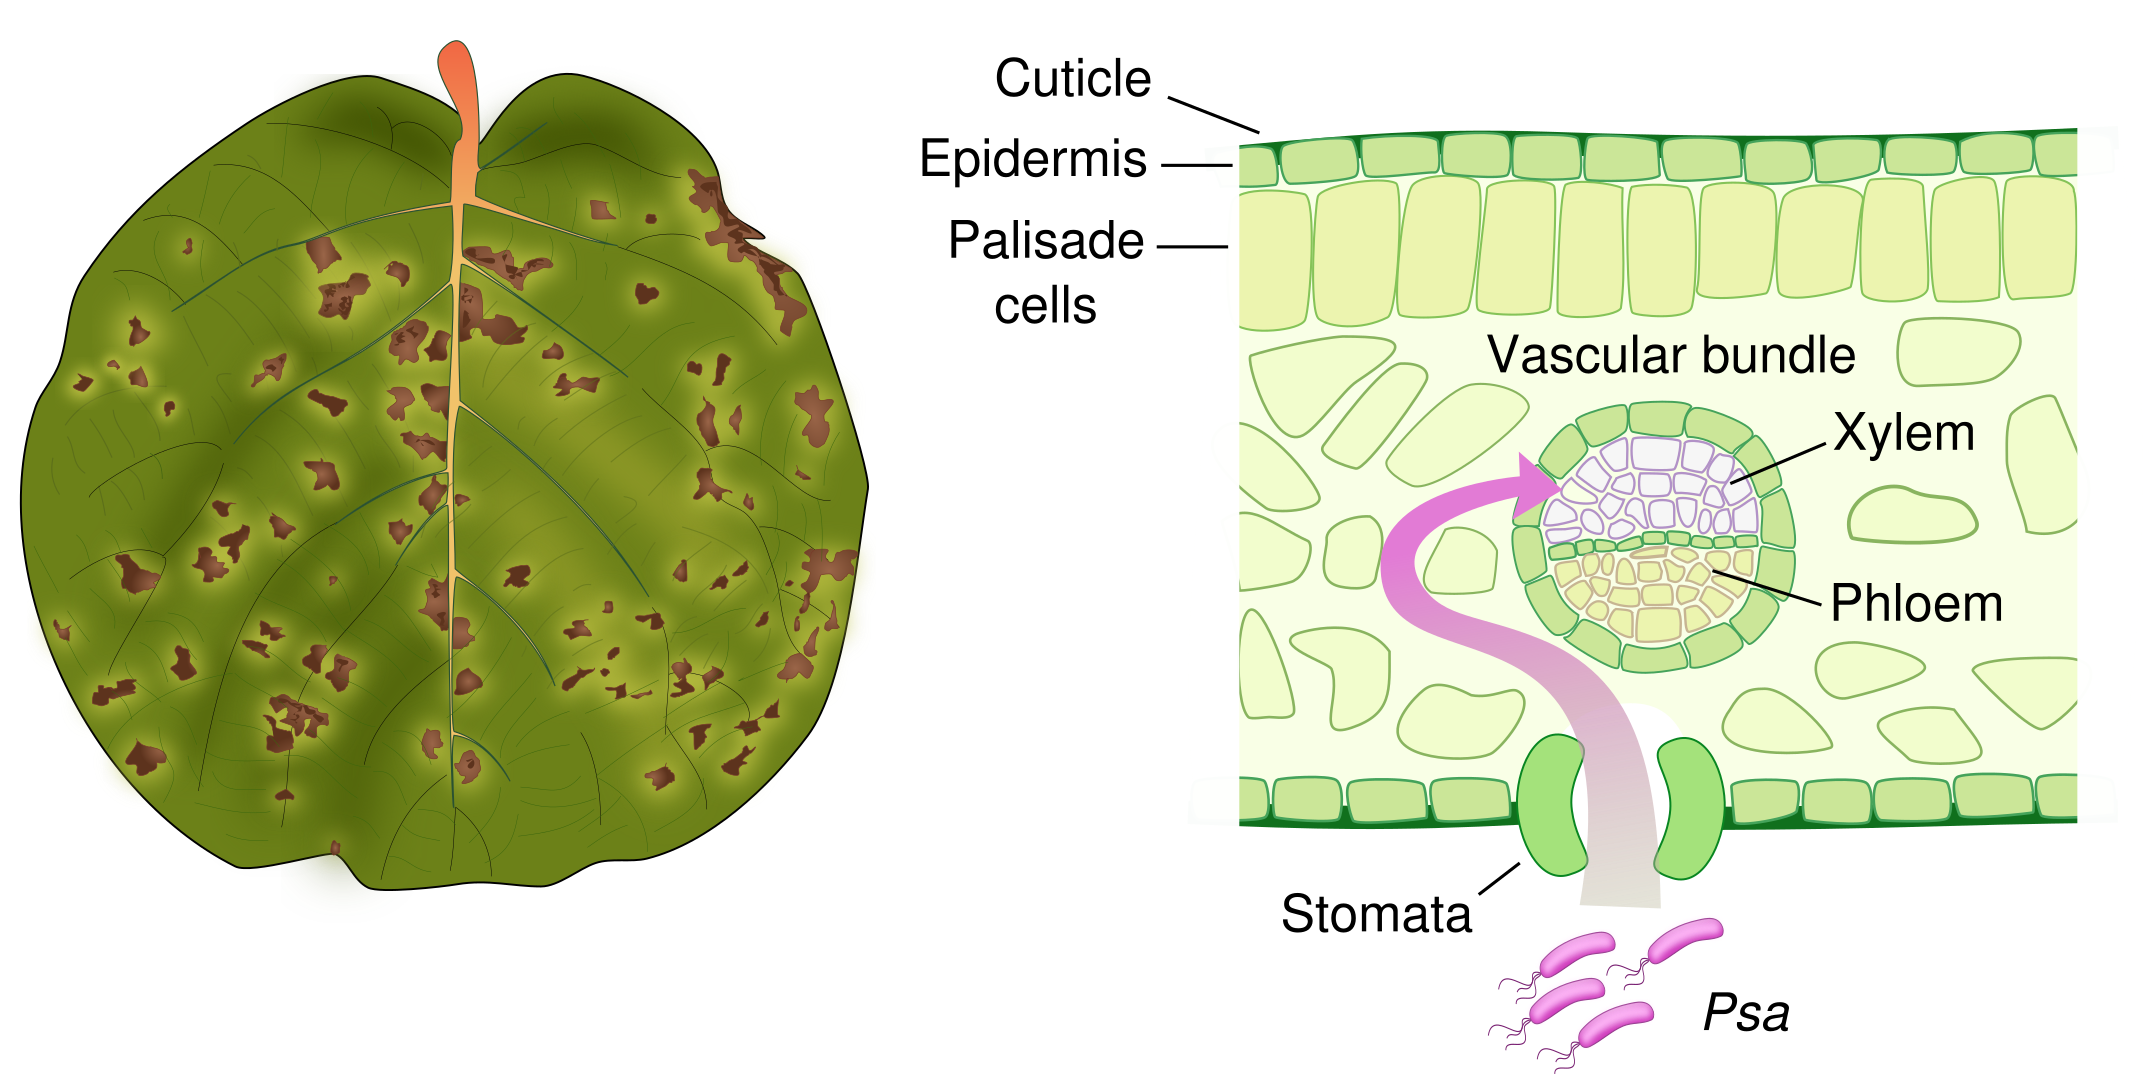
\includegraphics[scale=0.8]{psa/psa_infection.png}
  \centering
  \caption[Diagram showing \textit{Psa} infection of a kiwifruit leaf]{Diagram showing \textit{Psa} infection of a kiwifruit leaf. \textbf{Left:} Kiwifruit leaf infected by \textit{Psa}. Symptoms of the infection can be seen as brown patches of dead tissue caused by necrosis, as well as yellowing due to a loss of chlorophyll production in affected regions (chlorosis). \textbf{Right:} Potential avenue of \textit{Psa} infection of a leaf. \textit{Psa} enters through the stomata, and can reside in the apoplastic space where it triggers the plant necrotic response. \textit{Psa} may also make its way to a vascular bundle and enter the xylem to cause systemic infection.}
  \label{fig:psa_infection}
\end{figure}
Pathogenic strains of \textit{Pseudomonas syringae} utilise a type III secretion system (T3SS) to inject virulence factors into plant cells. These include effectors, proteins which interact and module host cells to promote pathogen survival. Like other plant pathogens, the T3SS locus of \textit{P. syringae} includes \textit{hrp} genes, a set of regulators, effectors and T3SS components that are activated in response to environmental stimuli \citep{Lindgren2003-ch}.

\textit{Hrp} genes are named after the ability of some \textit{hrp}-gene products to produce a hypersensitive response (HR) in the host plant. The HR is basal plant immune response which is characterised by ion flux and the generation of destructive free radicals, that cause local necrosis which helps to restrict the growth or spread of pathogens \citep{He_1996}. Virulence products produced by pathogens, such as effectors encoded by \textit{hrp} genes in \textit{P. syringae} \citep{He1993-zp,He_1996}, can trigger the HR response when these products are recognised by a cognate resistance (R) gene in the plant \citep{Keen_1990x}. These gene-for-gene responses can be unique to specific interactions between pathogens and hosts \citep{Heath_2000x}. Certain T3SS proteins and secreted compounds such as coronatine secreted by plant pathogenic bacteria can also act to suppress the plant HR by interfering with recognition pathways \citep{Nomura2005-dn}.

\subsection{Aims of this study}

Like other bacterial pathogens, \textit{Psa} experiences various levels of nutrient stress during infection and transmission. \textit{Pseudomonas syringae} pathogens famously can participate in the water cycle, enabling their spread to a wide range of aqueous environments and plant hosts by precipitation or splash contamination \citep{Morris_Monteil_Berge_2013x,Morris2008-szx,Hirano1990-sc}. 

Interestingly, \textit{P. syringae} appears to have evolved complementary adaptions to nutrient stress that optimise its survival and spread both in the environment and within plant hosts. Factors that enable \textit{P. syringae} to grow and spread in oligotrophic freshwater environments, such as metabolic versatility and the ability to sequester nutrients, are also associated with strain virulence and host range \citep{Morris_Monteil_Berge_2013x}.
For \textit{Psa} growing \textit{in planta}, the epiphytic stage of infection is likely to be nutrient poor with the exception of nectar \citep{Donati2018-fe}. Systemic infection within the xylem also requires adaption to a nutrient poor environment \citep{Vinatzer2012-nr} -- the uptake and utilisation of sucrose as a carbon source reported in \textit{Psa} may be an adaption to this. Bacteria in these environments are likely to face osmotic changes within different plant tissues, as well as oxidative stress from plant defence mechanisms \citep{Jones_Lindow_Wildermuth_2007,Nomura2005-dn}

For this study, \textit{Psa} was grown \textit{in vitro} in three culture mediums with different levels of nutrient availability, and transcriptomes generated for these mediums at different parts of the growth cycle. Comparisons of these transcriptomes highlights how \textit{Psa} adapts to nutrient stress, and identifies gene expression changes that may be relevant to survival and pathogenicity. These \textit{in vitro} transcriptomes were also compared with a recent \textit{in planta} study by \cite{McAtee2018-sl}, in which \textit{Psa} transcriptomes were generated over an infection time course of kiwifruit plantlets. 

%\textit{Questions} - What transcriptional changes occur between different growth medias and conditions - How does the \textit{in vitro} reflect the infection time-course? Are these these \textit{in vitro} growth conditions analagous to environments \textit{in planta}?
\section{Methods}
\subsection{\textit{In vitro} RNA-seq}

Cultures of \textit{Pseudomonas syringae} pv. \textit{actinidiae} isolate ICMP 18884 were grown in three different growth mediums at 20°C. Samples were grown in complete rich media (LB), with four replicates in log phase, and two in log/late log phase. In minimal media (M9 media supplemented with glucose), two samples were generated in log/late log phase, and four samples were generated under starvation conditions (0.1 M9 salts)
%Matt: unsure may have been AGRF
\begin{table}[H]
    \centering
    \footnotesize
    \begin{tabular}{cccccc}\toprule
Library & Name & Growth medium & Growth phase & OD A\textsubscript{600} & Ave. fragment size (bp) \\\midrule
2428_01 & M9-1 & Minimal & log/late log & 1.6 & 306 \\
2428_02 & M9-2 & Minimal & log/late log & 1.6 & 308 \\
2428_03 & LB-3 & Rich & late log & 4.6 & 306 \\
2428_04 & LB-4 & Rich & late log & 4.6 & 309 \\
2428_05 & ST-5 & Starved & NA & NA & 309 \\
2428_06 & ST-6 & Starved & NA & NA & 315 \\
2428_07 & LB-7 & Rich & log & 1.1 & 314 \\ 
2428_08 & LB-8 & Rich & log & 1.1 & 315 \\
2428_09 & LB-9 & Rich & log & 1.6 & 319 \\ 
2428_10 & LBA-10 & Rich & log & 1.6 & 311 \\
2428_11 & ST-11 & Starved & NA & NA & 326 \\
2428_12 & ST-12 & Starved & NA & NA & 318 \\
        \bottomrule
    \end{tabular}
    \caption[Summary of \textit{in vitro} RNA-seq libraries]{Summary of sequencing libraries and growth conditions of the twelve \textit{in vitro} \textit{Psa} RNA-seq samples. Three growth mediums were used: Rich (LB media), Minimal (M9 media supplemented with glucose) and Starved (0.1 M9 salts). Growth phase was determined by measuring optical density/absorbance at 600 nm (OD A\textsubscript{600}). Growth phase could not could not be reliably determined for starved samples due to a lack of bacterial growth in this medium. Average fragment size of RNA libraries ranged from 306--326 nt across the samples. }
        \label{table:in_vitro_sequencing_summary}
\end{table}

RNA was extracted using an Ambion Pure kit. Ribosomal rRNA depletion was performed by New Zealand Genomics Limited (NZGL) using an Illumina Ribo-Zero rRNA Removal Kit. All libraries for the project were stranded and sequenced on a single Hi-Seq cell.

\subsection{Differential gene expression}
Raw reads were processed with \texttt{trimmomatic} \citep{Bolger2014-ob} to remove adaptors and regions of poor quality sequence. Transcripts for all \textit{Psa} genes
%nb all IYOs, which includes ncRNAs such as RNAseP
were quantified using \texttt{Kallisto} \citep{Bray2016-oi} and count data analysed using \texttt{DESeq2} \citep{Love2014-dv}. The full data analysis pipeline is provided as a jupyter notebook in the supplemental materials (Appendix X).

\subsection{Pathway analysis}
\texttt{Pathview} \citep{Luo_Brouwer_2013} was used to visualise the overall effect of growth condition on gene expression. KEGG annotations for orthologous genes from \textit{Pseudomonas syringae} pv. \textit{tomato} DC3000 (\textit{PSPTO}) were used for pathway analysis. Orthologous genes were annotated using a \texttt{blastp} \citep{Altschul1990-dkr} search of \textit{Psa} proteins against \textit{PSPTO} proteins, and taking the highest-scoring significant result for each \textit{Psa} protein (E-value threshold 0.05). Pathways containing more than nine highly differentially expressed genes were visualised with \texttt{Pathview} (Appendix X). 

For pathways with multiple genes mapping at the same node, the gene with the largest total change in gene expression across all media comparisons was used. Mapped \textit{Psa} genes were renamed by their IYO gene number on the plots generated by \texttt{Pathview} using a custom Perl script. Log\textsubscript{2} fold-change for each comparison (rich vs starved, rich vs minimal, minimal vs starved) were plotted on each node as a heatmap, ranging from -8 (dark blue) to 8 (deep red).

\subsection{Functional annotation}

A set of comprehensive functional annotations was created for predicted protein-coding genes in the \textit{Psa} genome and plasmid (NCBI accessions$:$ CP011792.2 and CP011793.1) \citep{Templeton2015-ma}. Proteins were functionally annotated using the EggNOG web server \citep{Huerta-Cepas2017-xmpx}. Secondary metabolites were predicted using the antiSMASH web server\citep{Medema2011-ub}. RAST \citep{Aziz2008-eh} annotations, and a set of custom annotations were also provided by Matt Templeton.

\subsection{Comparison to \textit{in planta} data}
RNA-seq data from \cite{McAtee2018-sl} was obtained from the NCBI Sequence Read Archive (SRA) project SRP148711 (Table \ref{table:1}). Raw reads from samples infected with \textit{Psa} at different time-points were downloaded and processed using the same analysis pipeline as the \textit{in vitro} RNA-seq.
\begin{table}[H]
\footnotesize
    \centering
    \begin{tabular}{ccccc}\toprule
Time-point & SRA Accession \\\midrule
1.5hrs & SRR7204724 & SRR7204725 & SRR7204726 \\
3hrs & SRR7204727 & SRR7204728 & SRR7204729 \\
6hrs & SRR7204688 & SRR7204694 & SRR7204707 \\
12hr & SRR7204687 & SRR7204689 & SRR7204708 \\
24hrs & SRR7204690 & SRR7204691 & SRR7204693 \\
48hrs & SRR7204692 & SRR7204695 & SRR7204706 \\
72hrs & SRR7204685 & SRR7204686 & SRR7204711 \\
96hrs & SRR7204709 & SRR7204710 & SRR7204712 \\
120hrs & SRR7204713 & SRR7204714 & SRR7204715 \\
        \bottomrule
    \end{tabular}
    \caption[\textit{In planta} RNA-seq samples]{Time-points and SRA accessions for \textit{in planta} RNA-seq samples}
    \label{table:1}
\end{table}

\section{Results and Discussion}

\subsection{RNA-seq quality control}

\subsubsection{\textit{In vitro} samples}

Approximately 60\% of all \textit{in vitro} sequencing reads (approximately 10 million counts per sample) were successfully mapped to protein coding genes (Table \ref{tab:in_vitro_mapping}). During initial quality control, it was found that ribosomal RNA depletion for Sample 10 had failed. This sample was not included in further analyses.

Principal component analysis (Figure \ref{fig:PCA_plot}) showed that \textit{in vitro} samples clustered by media and growth phase, with the majority of variance in PC1 due to growth medium, with some variance between the two distinct growth phases in the rich media samples in PC2. Starved samples showed some within-group variance, which may be due to differences in growth phase.

Hierarchical clustering of sample-to-sample distances (Figure \ref{fig:hierarchical_clustering}) showed strong within-group similarity for media type and growth phase, with starved samples showing the same within-group variation observed in the principal component analysis (Figure \ref{fig:PCA_plot}. Samples grouped primarily by growth phase instead of media type. Rich media samples formed two separate clusters based on growth phase. Starved samples were closest to rich media samples in log/late log phase, which may be due to similarities in growth limitation in these samples. Minimal media samples were most similar to the rich media samples in log phase. 
\begin{table}[H]
\footnotesize
    \centering
    \begin{minipage}{0.75\textwidth}
    \begin{tabular}{ccccc}\toprule
    Sample & Sample name & Total counts & \% Reads mapped to genes\\\midrule
Sample_1 & M9-1 & 10560672 & 60.3 \\
Sample_2 & M9-2 & 10248103 & 58.9 \\
Sample_3 & LB-3 & 8416904 & 49.1 \\
Sample_4 & LB-4 & 8707835 & 49.8 \\ 
Sample_5 & ST-5 & 9370257 & 52.8 \\
Sample_6 & ST-6 & 9965784 & 58.7 \\
Sample_7 & LB-7 & 10435416 & 64.0 \\
Sample_8 & LB-8 & 10886018 & 66.8 \\
Sample_9 & LB-9 & 11590564 & 67.4 \\
Sample_10 & LBA-10 & 8703562 & 51.6 \\ 
Sample_11 & ST-11 & 10249949 & 57.7 \\
Sample_12 & ST-12 & 9256567 & 58.6 \\
\bottomrule
    \end{tabular}
    \end{minipage}
    \begin{minipage}{0.24\textwidth}
        \caption[\textit{In vitro} read mapping statistics]{Number of RNA-seq transcripts for \textit{in vitro} samples. Growth medium and phase associated with sample names are detailed in Table \ref{table:in_vitro_sequencing_summary}). The overall proportion of reads mapping to \textit{Psa} transcripts for each sample range from 49.1--67.4\%}
    \label{tab:in_vitro_mapping}
    \end{minipage}
\end{table}
\hfill
\begin{figure}[H]
  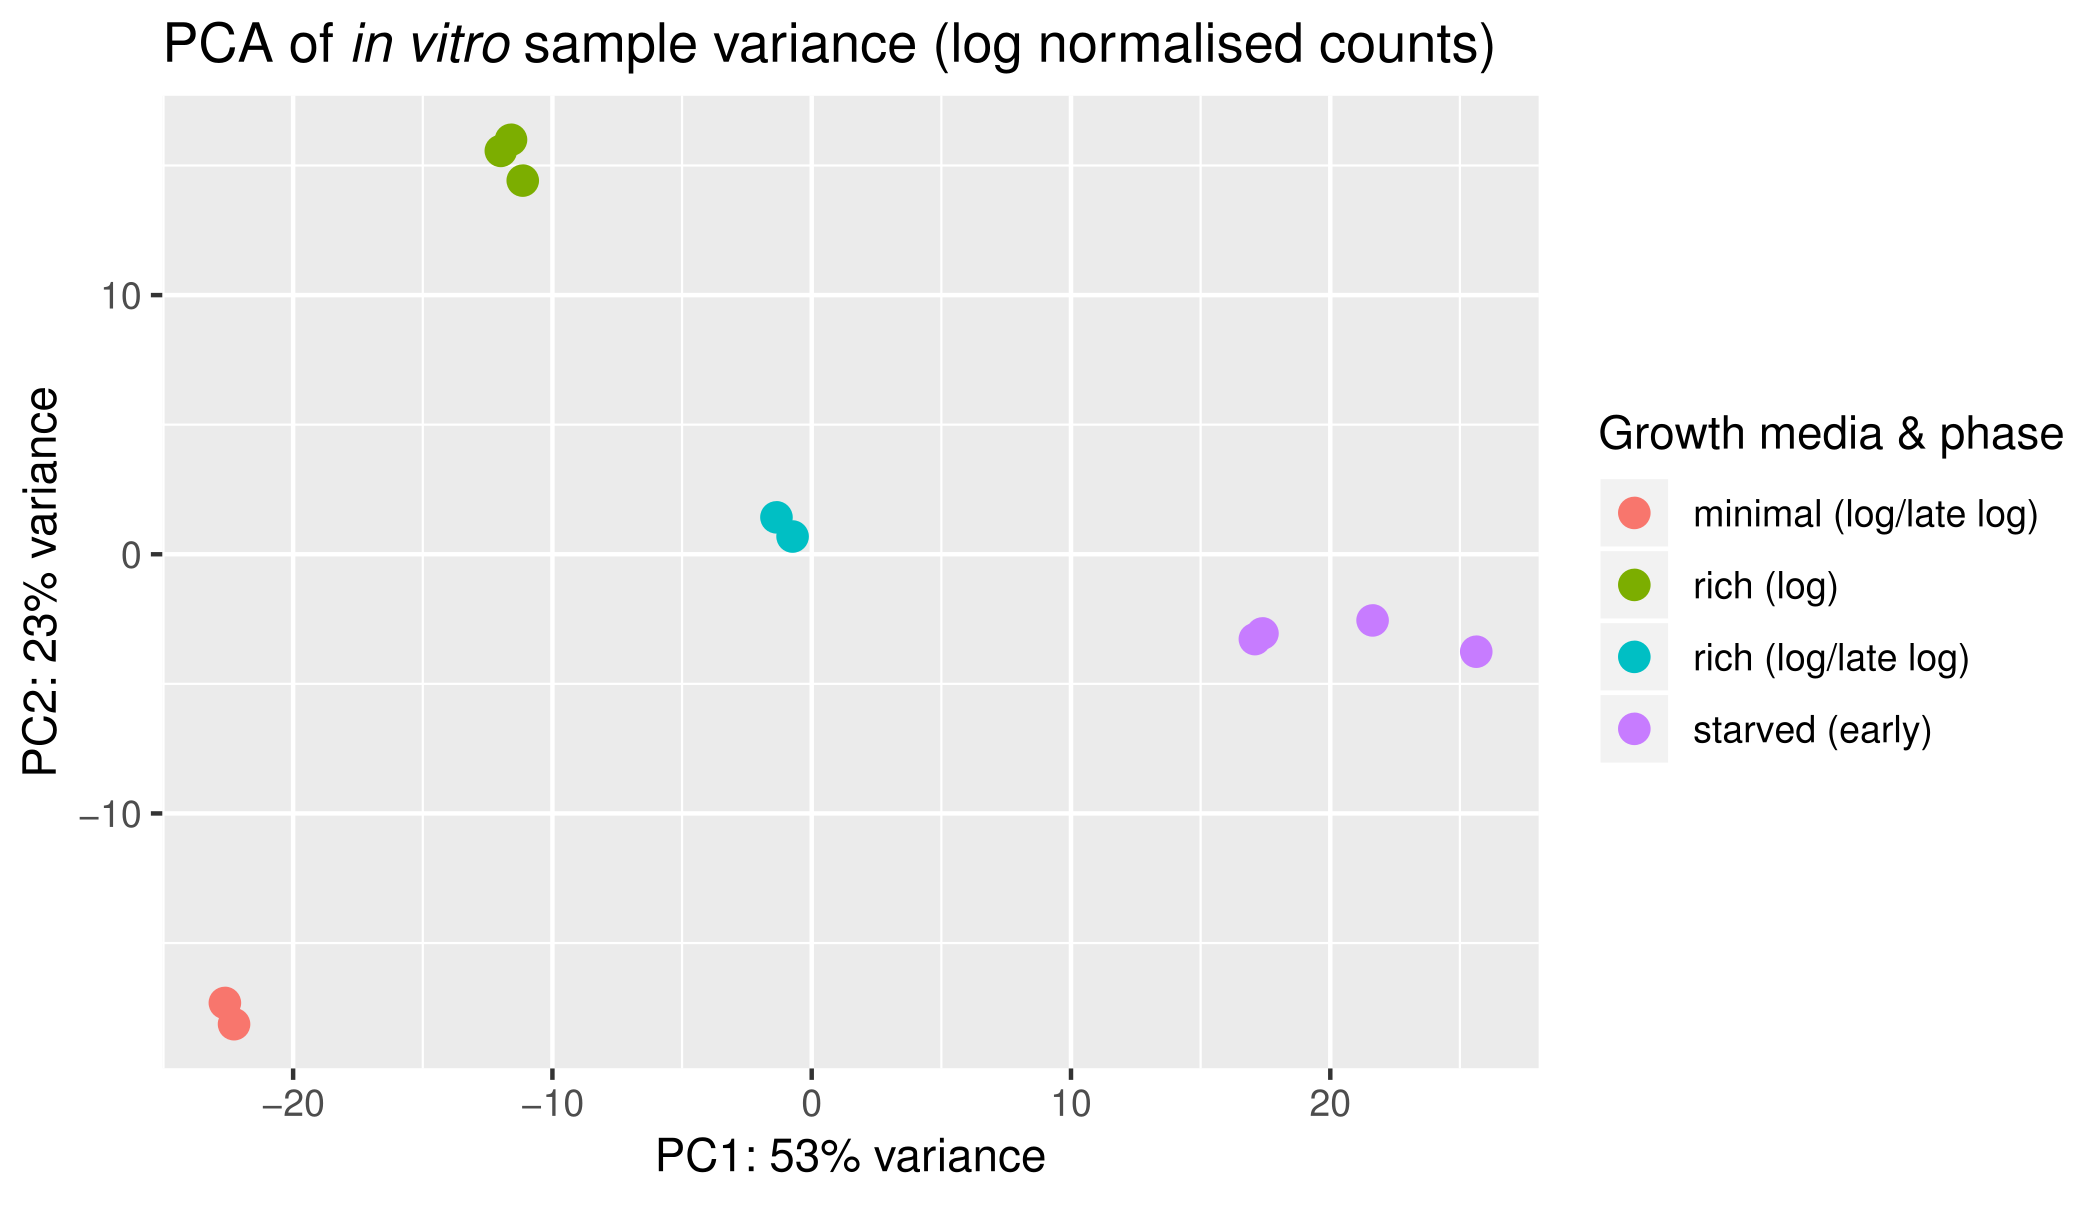
\includegraphics[scale=0.85]{psa/PCA_final_samples.png}
  \centering
  \caption[PCA plot of \textit{in vitro} samples]{Principal component analysis of gene expression data (log\textsubscript{2} normalised counts) from \textit{in vitro} samples. Sample-sample distances are plotted along the first two principal components (PC1 and PC2). Points represent individual samples, which are coloured by experiment group (growth medium and growth phase). Samples clustered by experiment type along PC1 and PC2, showing similarity between replicates. Sample groups were distinct and well separated across both principal components.}
  \label{fig:PCA_plot}
\end{figure}


\begin{figure}[H]
  \centering
    
\includegraphics[width=\textwidth]{psa/sample_distances_combo_final.png}
  \caption[Hierarchical clustering of \textit{in vitro} RNA-seq samples]{Heatmap showing sample-sample distances between \textit{in vitro} samples after hierarchical clustering, based on DESeq2 normalised counts. Replicate samples are clustered into groups showing high similarity to each other. Sample groups are then clustered by growth phase and media type.}
  \label{fig:hierarchical_clustering}
\end{figure}

An MA-plot visualising the log\textsubscript{2} fold change (l\textsubscript{2}FC) compared to the mean of normalised counts for all genes in the \textit{in vitro} samples showed that that few genes had low expression overall, and that the majority of genes were differentially expressed across the data-set. Overall, 2592/5809 genes had a l\textsubscript{2}FC with p < 0.01, and 2649/5809 genes had a l\textsubscript{2}FC with p < 0.0001 (Figure \ref{fig:in_vitro_MA_plot}).

Histograms showing the frequency distribution of Benjamini-Hochberg adjusted P values (P\textsubscript{adj}) for log\textsubscript{2} fold changes for pairwise comparisons of sample types showed 500-1000 differentially expressed genes (DEGs) with a P\textsubscript{adj} < 0.01 for each comparison (Figure \ref{fig:hist_growth}, Figure \ref{fig:hist_media}). Comparisons between growth phases showed many genes were highly differentially expressed between rich media samples -- rich media samples were also more different to each other than to the minimal media sample. Rich media log phase samples were most similar to minimal media log/late log phase samples.

Comparisons between media types showed rich media samples overall were most similar to minimal media samples, with only 522 DEGs P\textsubscript{adj} < 0.01. Approximately 1500 genes were highly differentially expressed (P\textsubscript{adj} < 0.0001) in comparisons between the starved samples and the other media types, whereas only 257 genes were differentially expressed between rich and minimal media samples (Table \ref{tab:sig_DEGs}).

\begin{figure}[H]
    \centering
    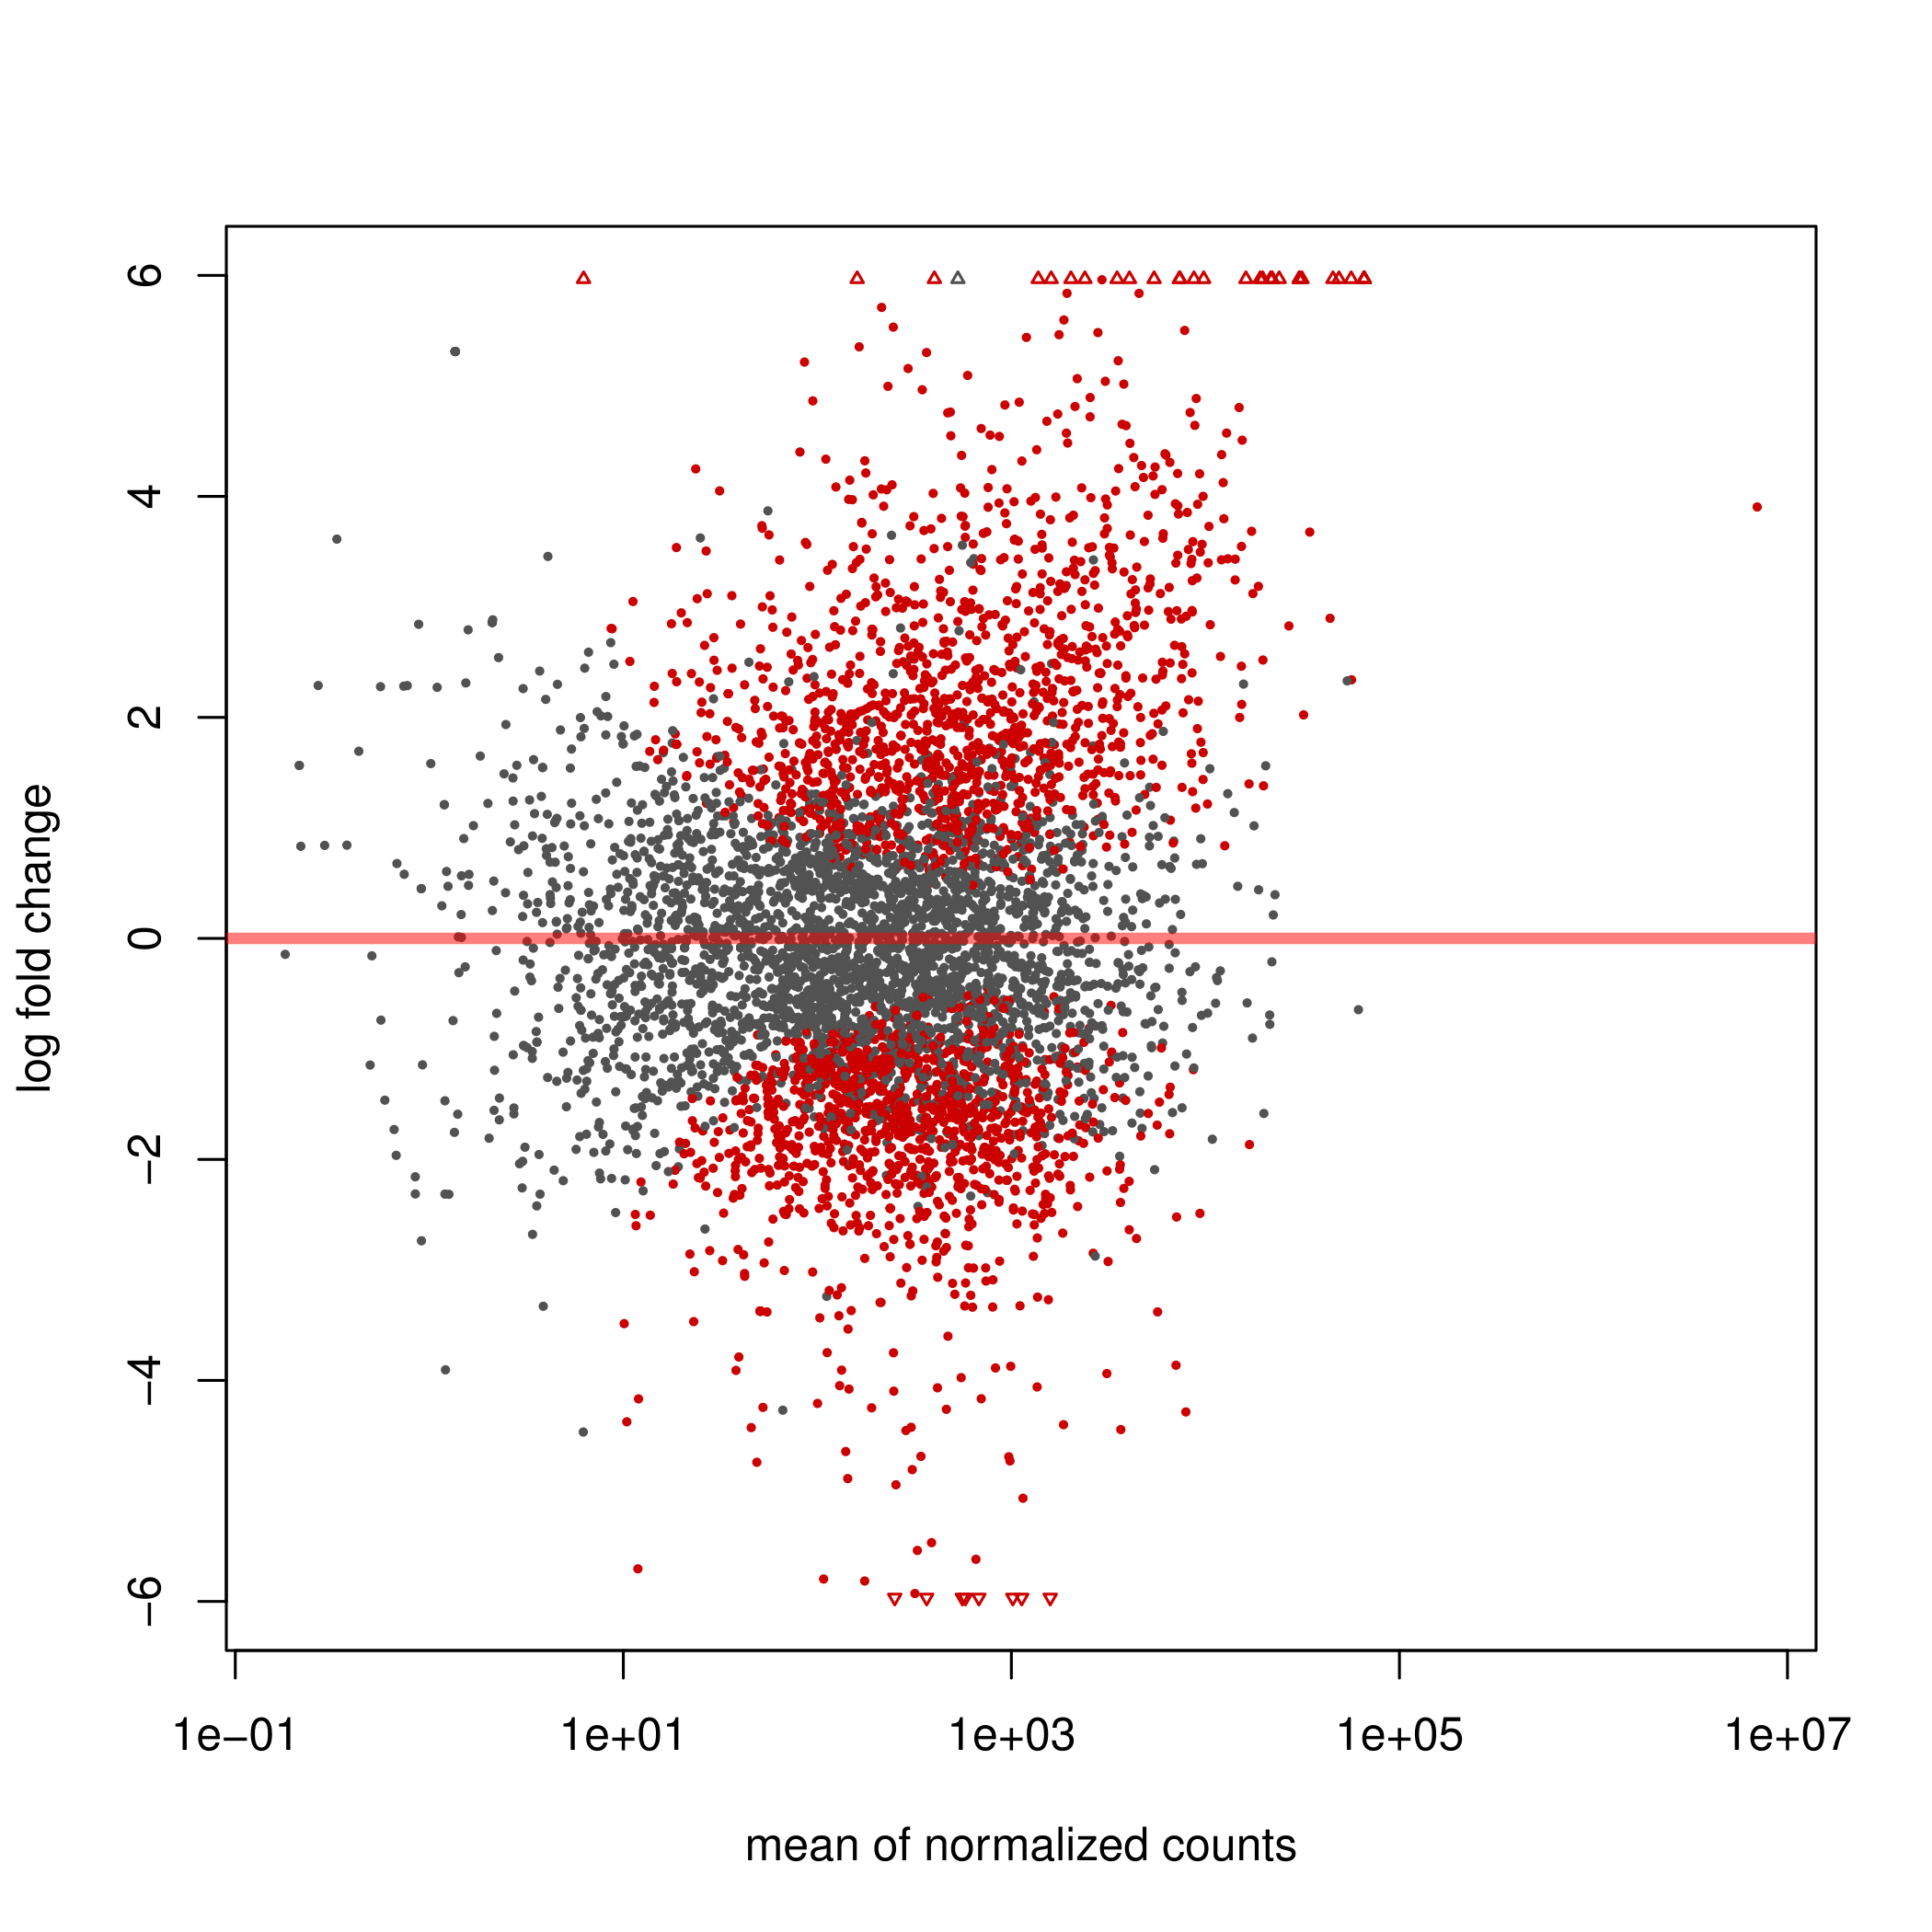
\includegraphics[scale=0.8]{psa/MA_plot_final_samples.png}
    \caption[MA-plot of gene expression changes for \textit{in vitro} experiments]{MA-plot showing the log\textsubscript{2} fold changes (l\textsubscript{2}FC) compared to the mean of normalised counts for all genes in the \textit{in vitro} samples. Genes with a highly significant l\textsubscript{2}FC (p < 0.0001) are highlighted in red. Plot generated using \texttt{DESeq2}.}
    \label{fig:in_vitro_MA_plot}

\end{figure}


\begin{table}[H]
\begin{minipage}{0.7\textwidth}
    \centering
    \begin{tabular}{cccc}\toprule
Sample type & Starved & Minimal & Rich (log) \\\midrule
Starved  & - & - & - \\
Minimal & 1561 & - & - \\
Rich (all) & 1572 & 257 & - \\
Rich (log) & 2694 & 651 & - \\
Rich (log/late log) & 1878 & 1368 & 1590 \\\bottomrule
    \end{tabular}
    \end{minipage}
    \begin{minipage}{0.29\textwidth}
    \caption[Numbers of significantly expressed genes for in vitro sample comparisons]{Numbers of highly differentially expressed genes for pairwise comparisons of \textit{in vitro} experiment factors (P\textsubscript{adj} < 0.0001)	}
    \label{tab:sig_DEGs}
        \end{minipage}
\end{table}


\begin{figure}[H]
\begin{subfigure}{0.49\textwidth}
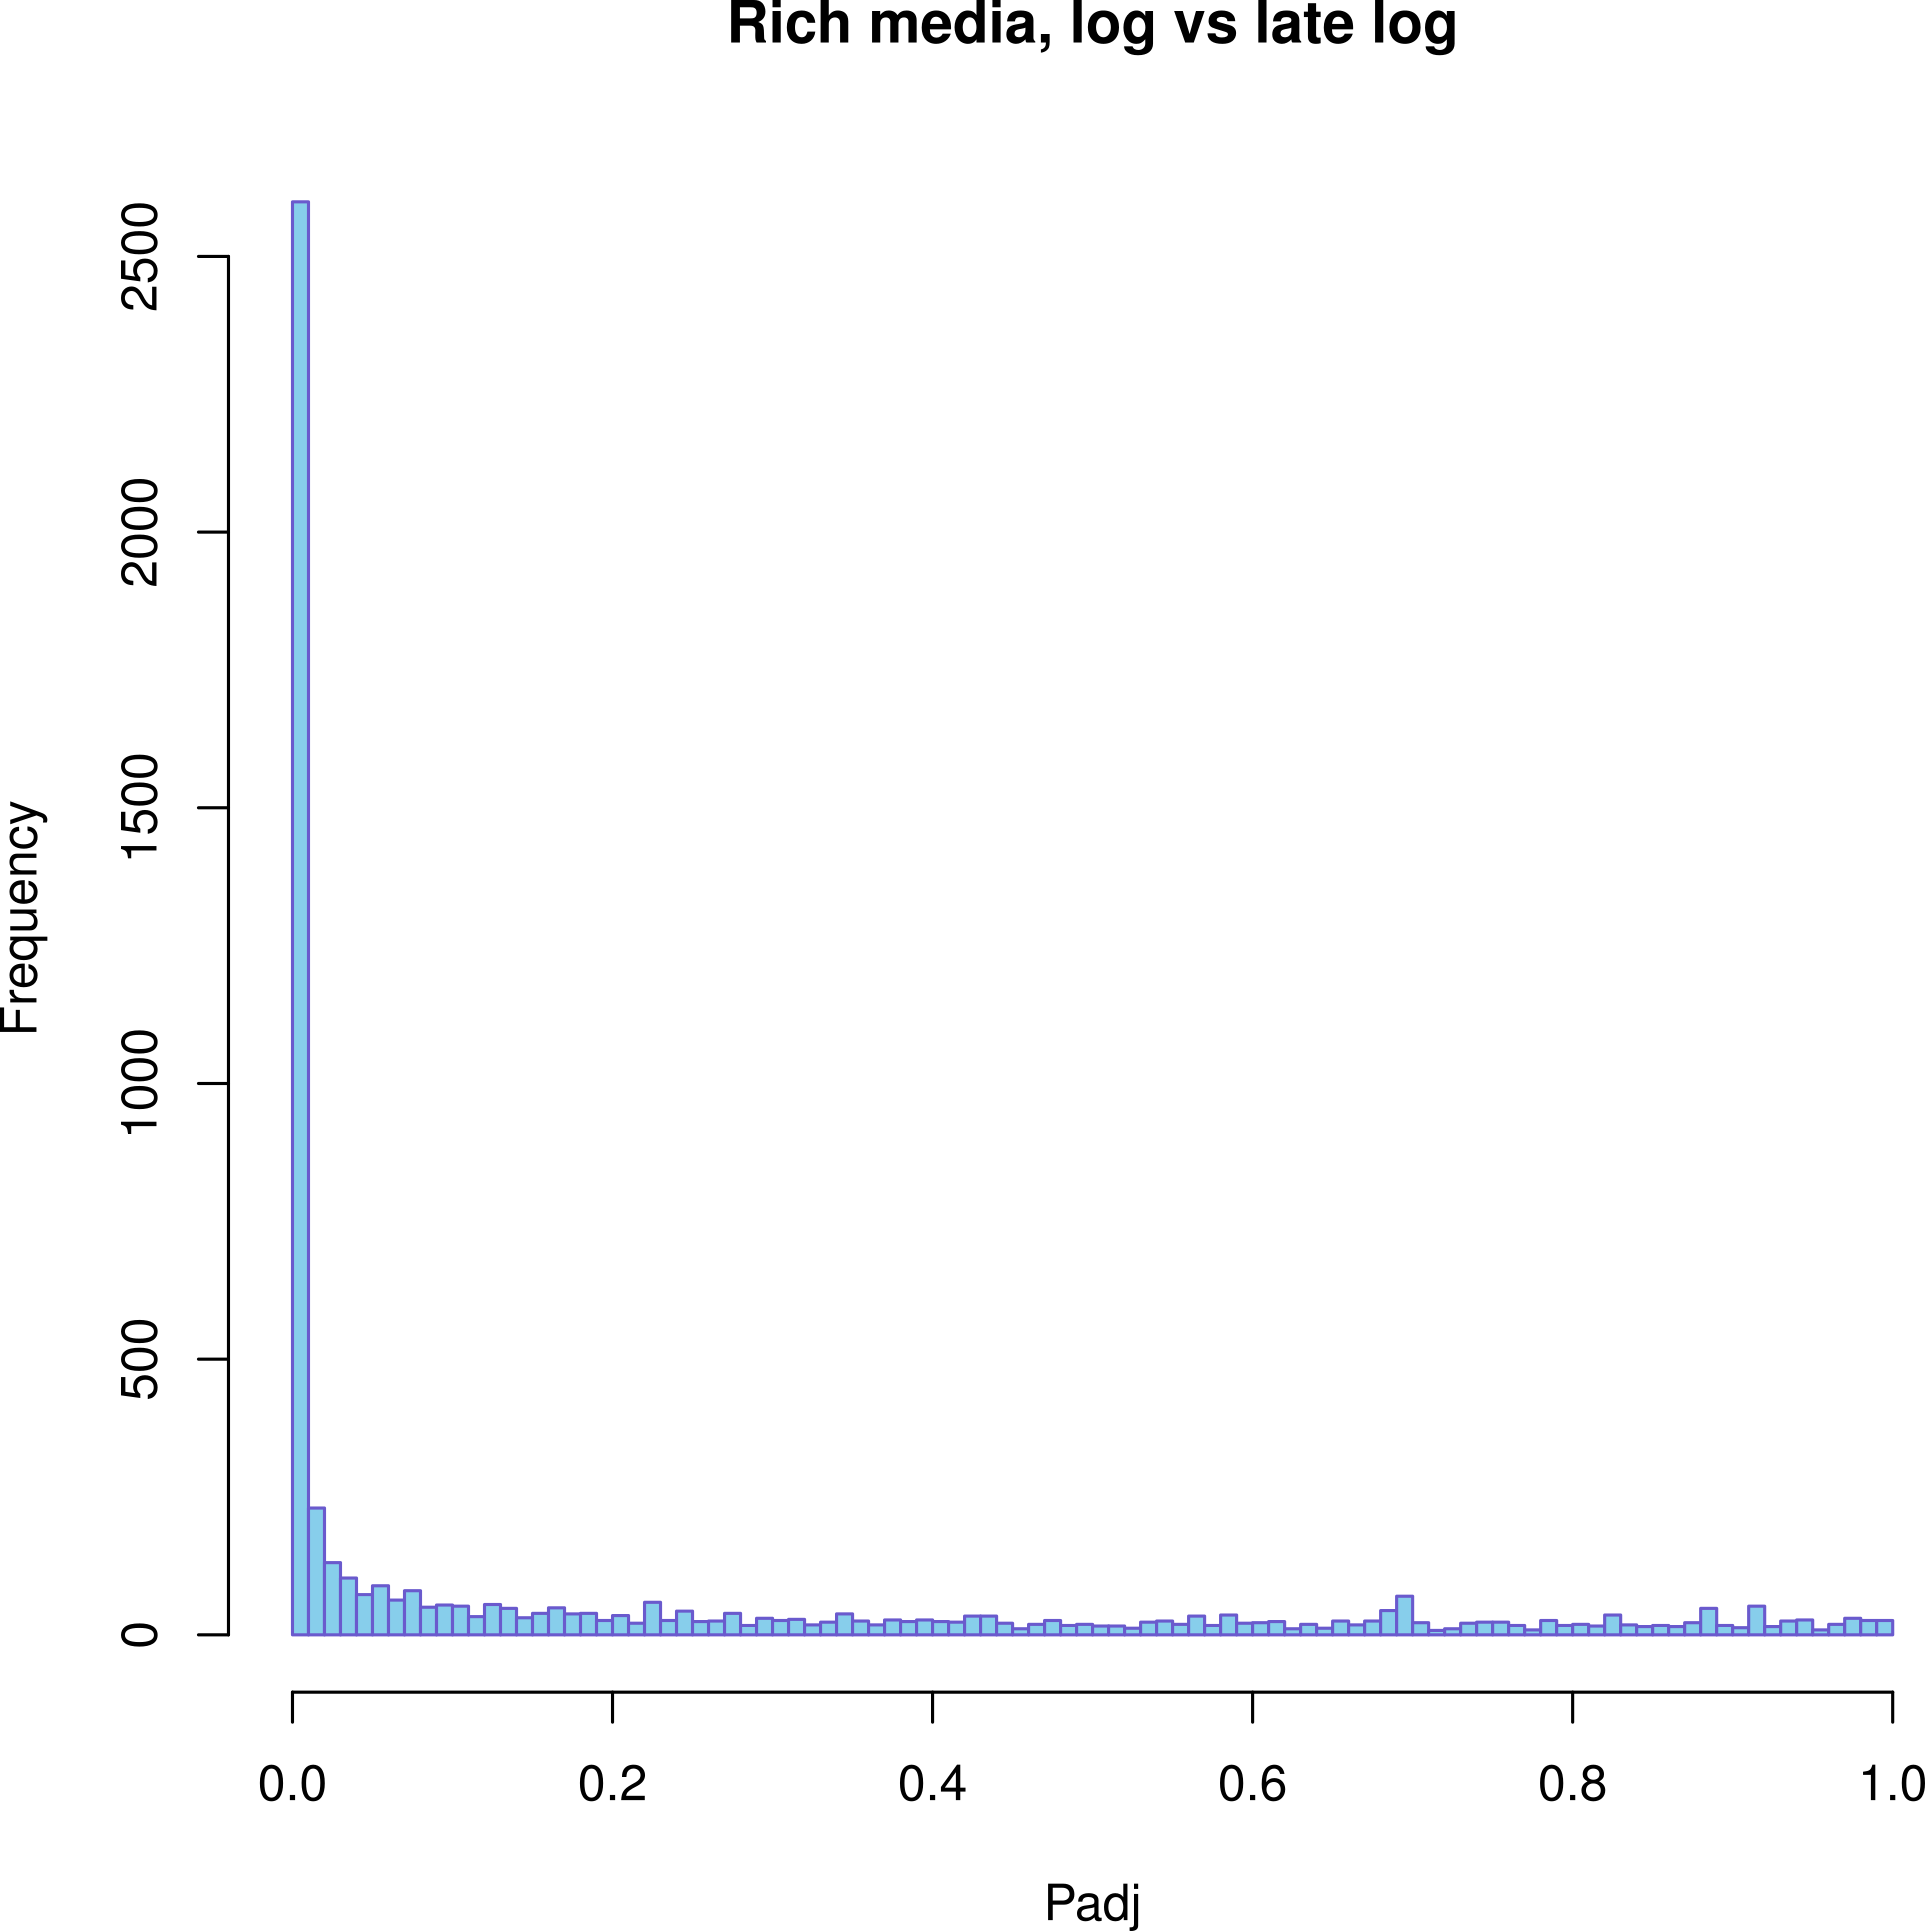
\includegraphics[width=0.9\linewidth]{psa/hist_richlog_richloglate.png} 
\end{subfigure}
\begin{subfigure}{0.49\textwidth}
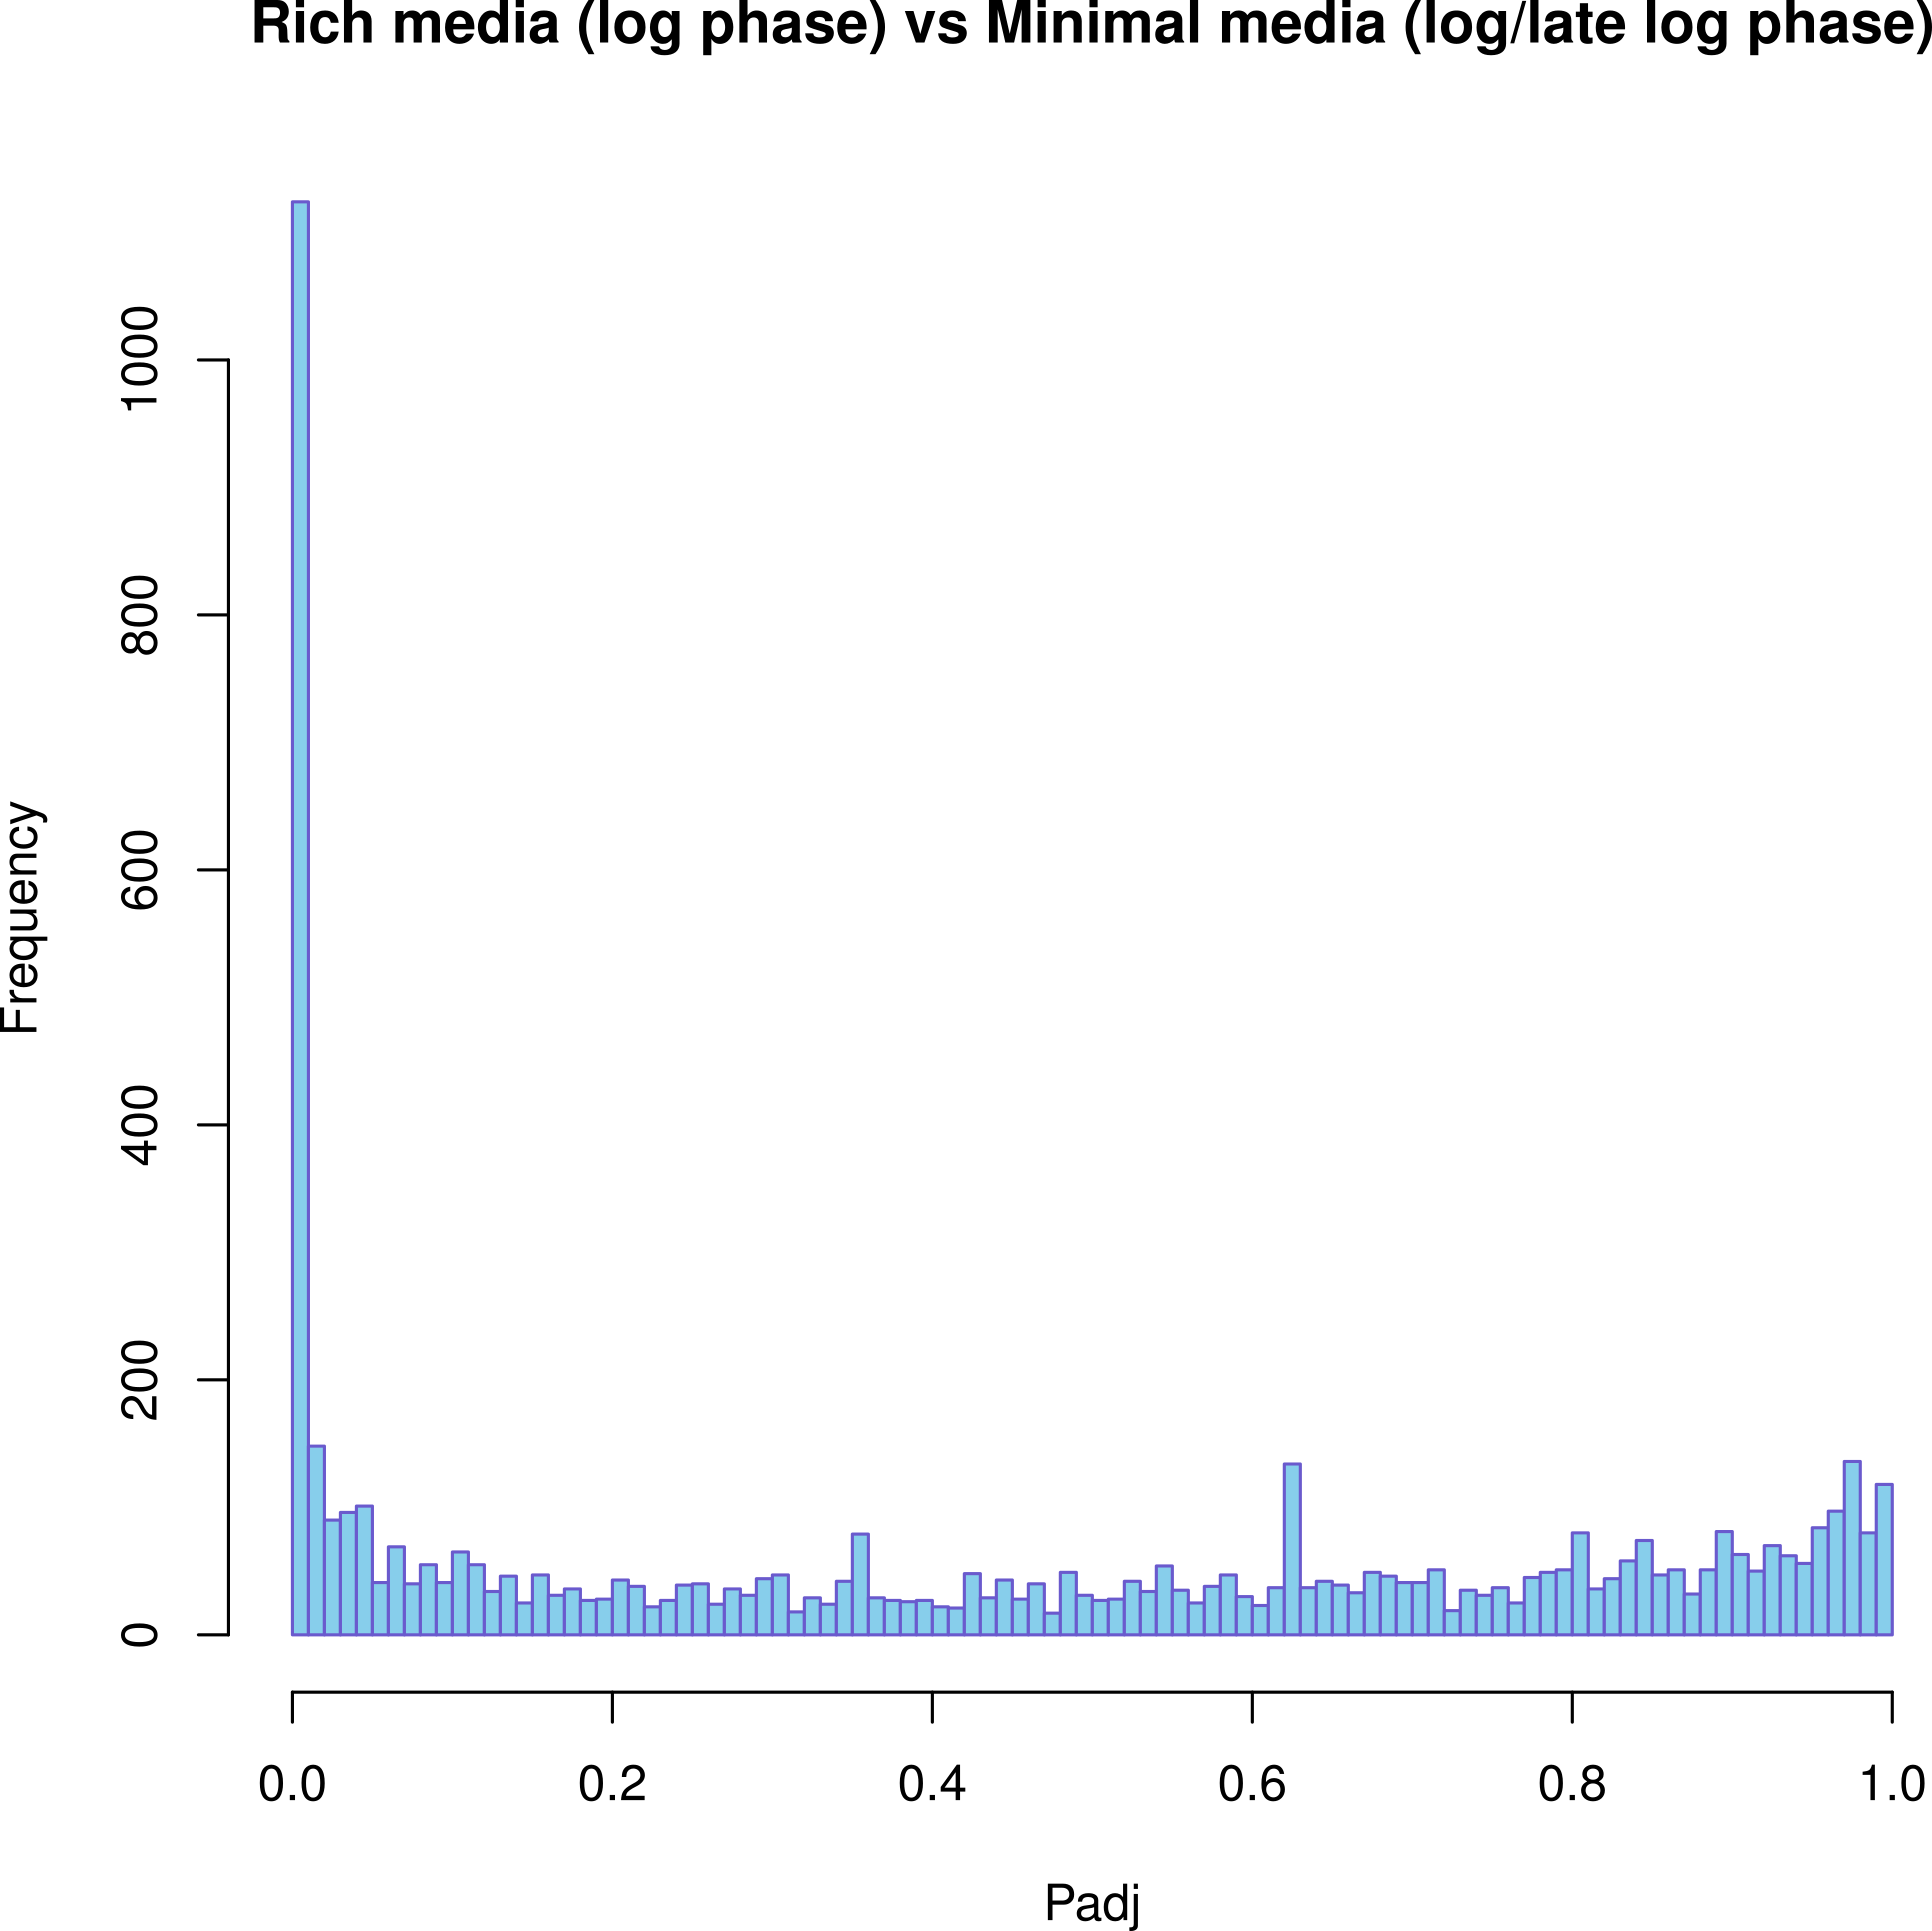
\includegraphics[width=0.9\linewidth]{psa/hist_richlog_minimal.png}
\end{subfigure}
\begin{subfigure}{0.49\textwidth}
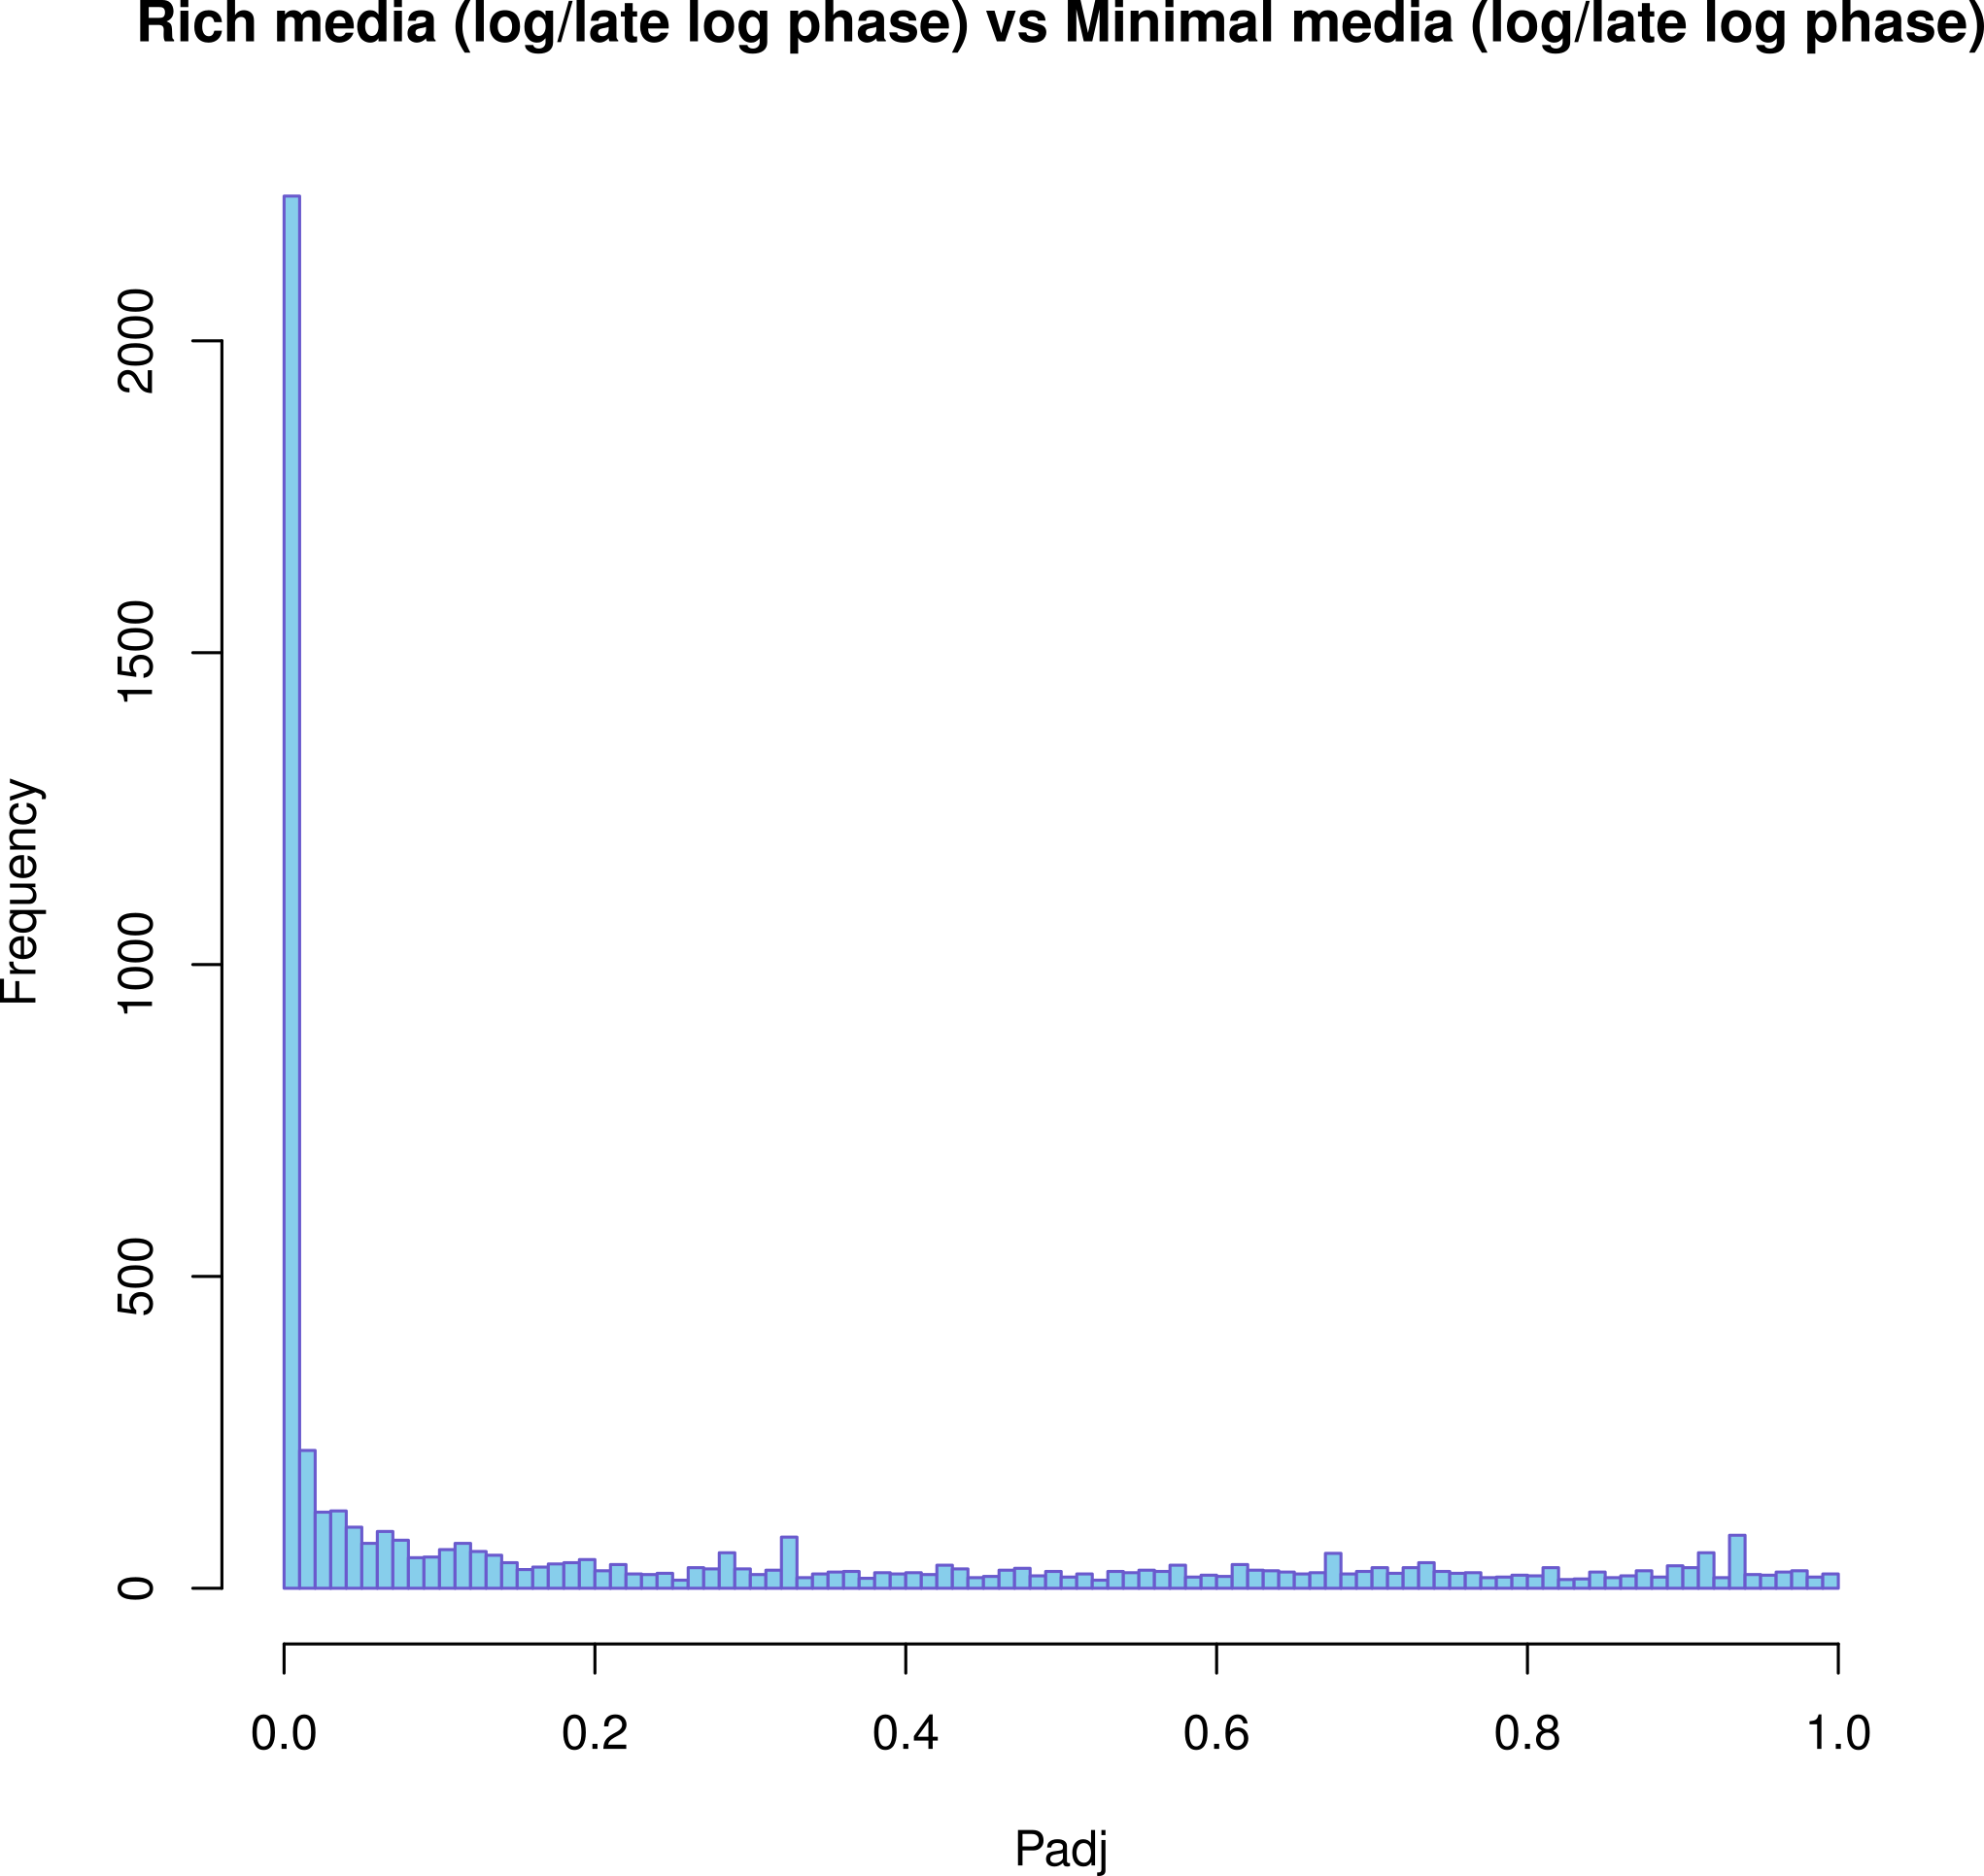
\includegraphics[width=0.9\linewidth]{psa/hist_richloglate_minimal.png}
\end{subfigure}
\begin{subfigure}{0.49\textwidth}
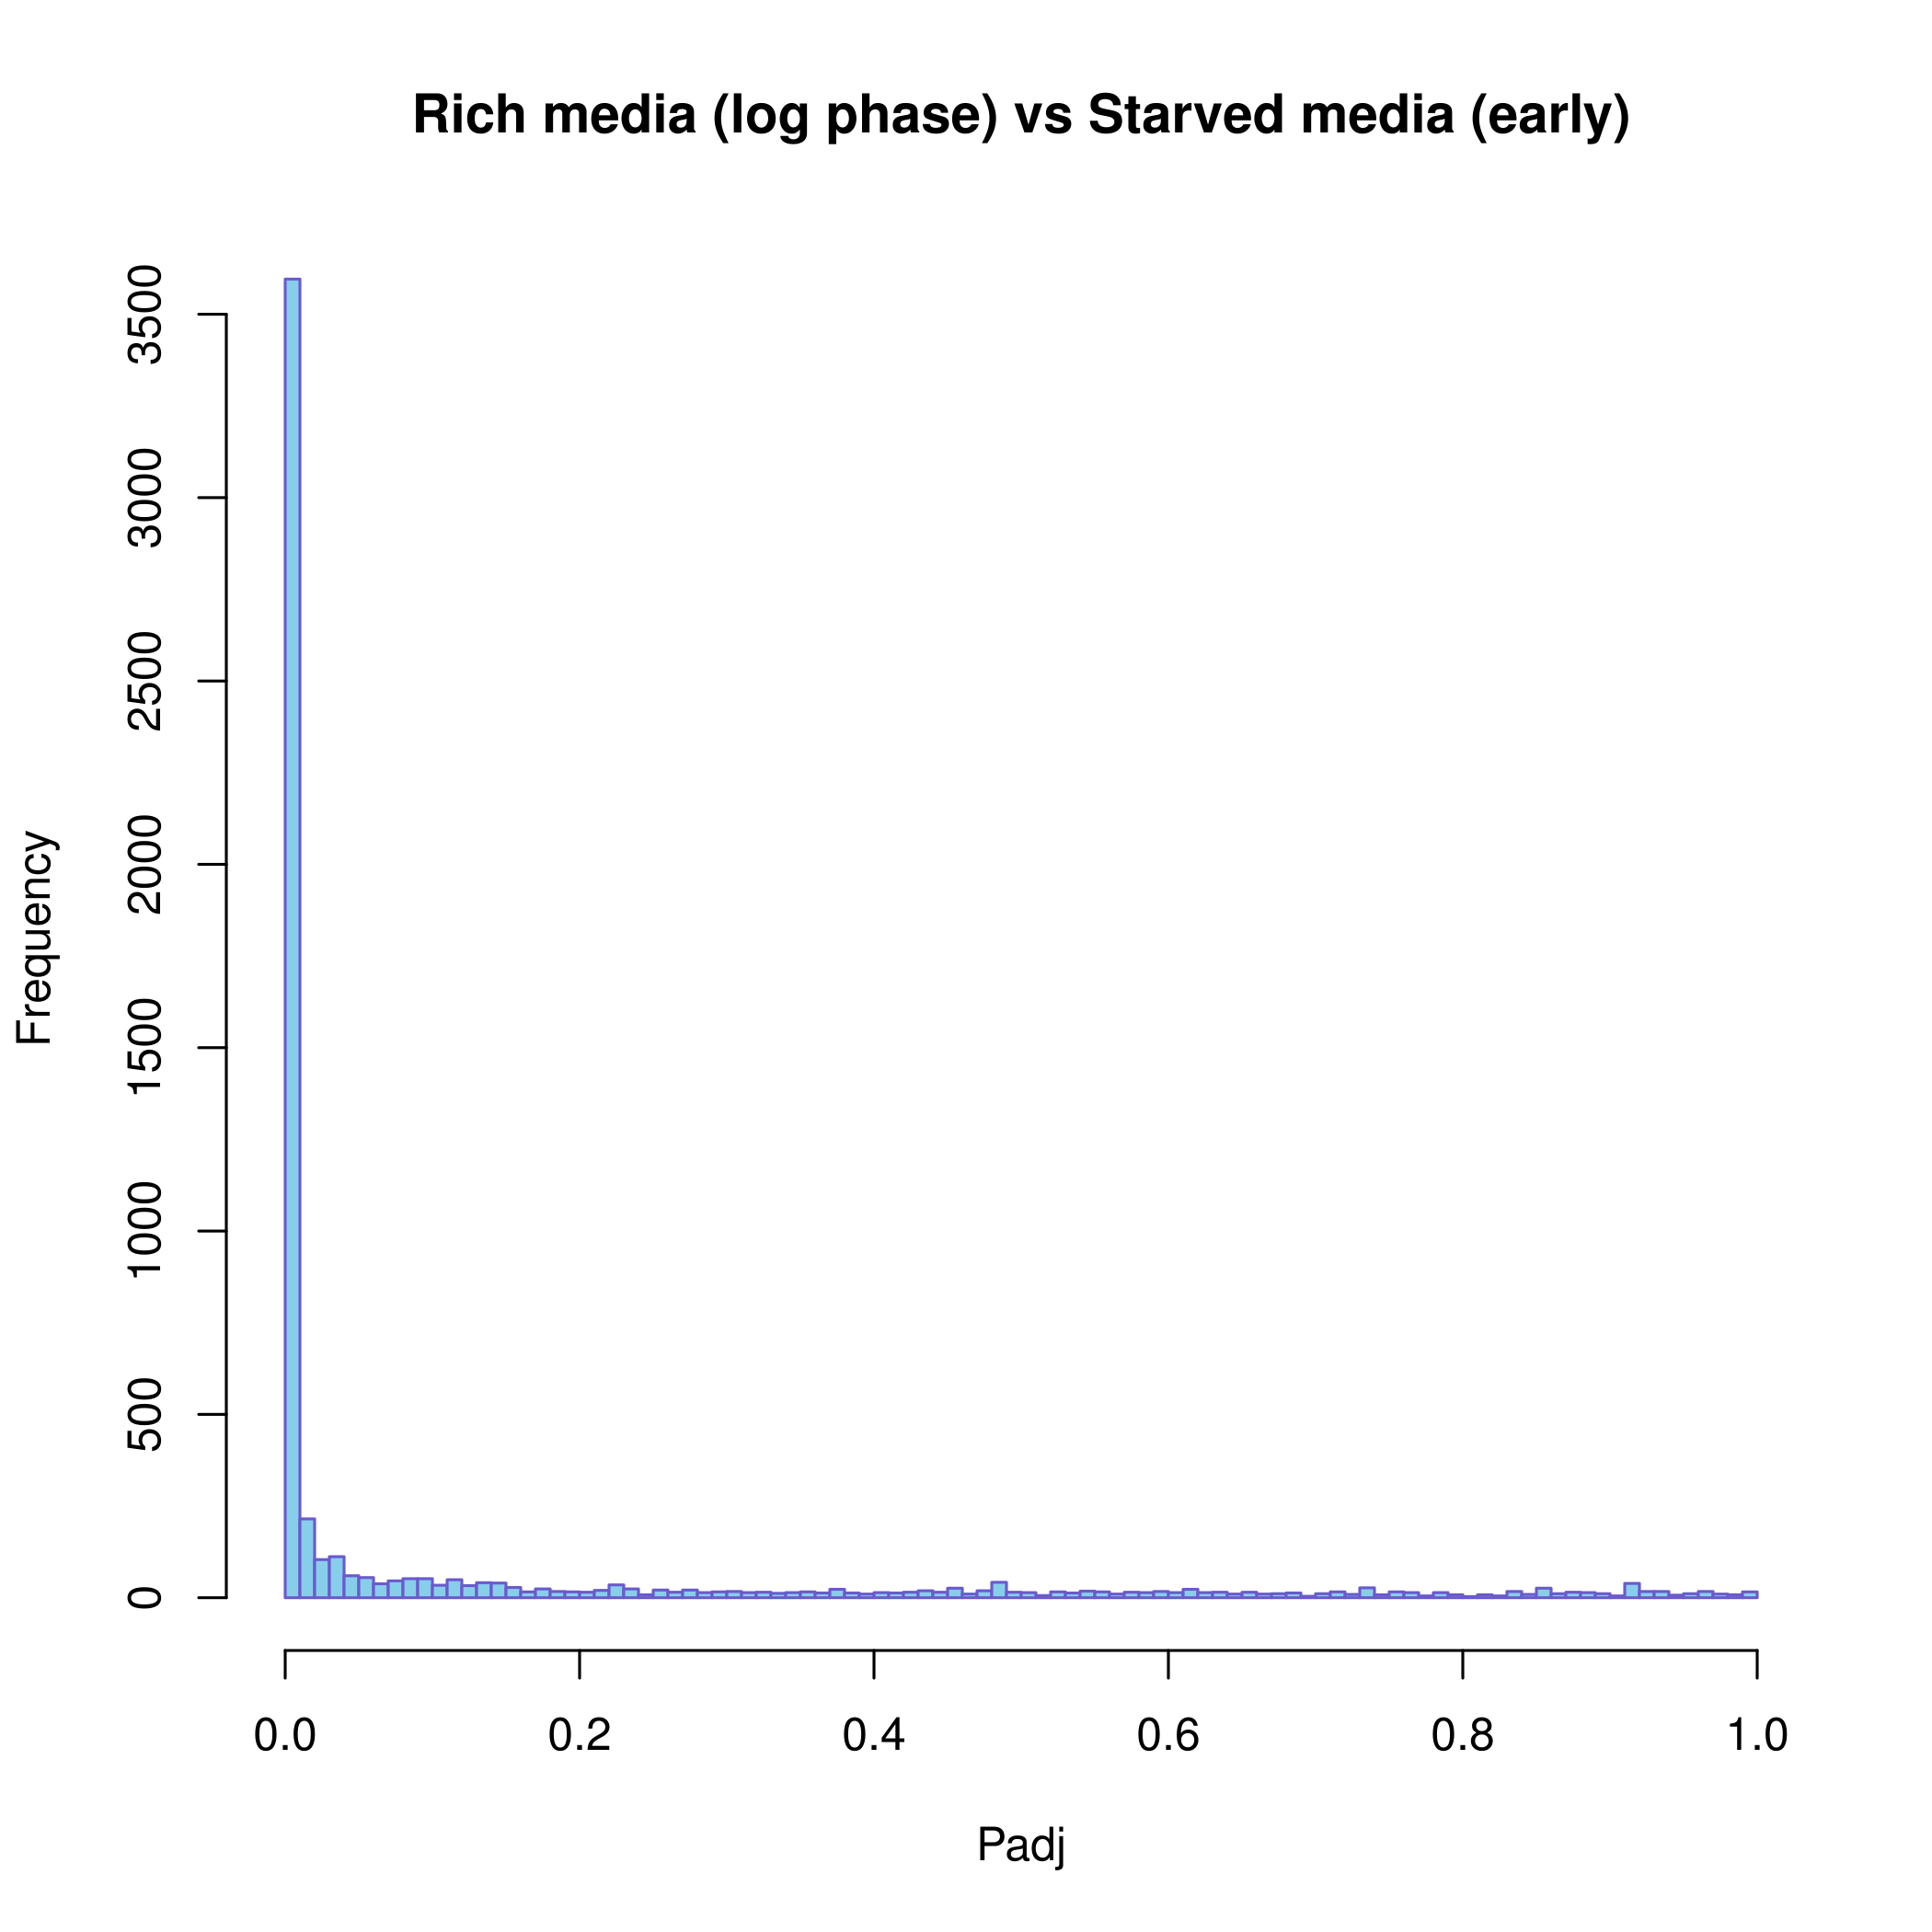
\includegraphics[width=0.9\linewidth]{psa/hist_richlog_starved.png}
\end{subfigure}
\begin{subfigure}{0.49\textwidth}
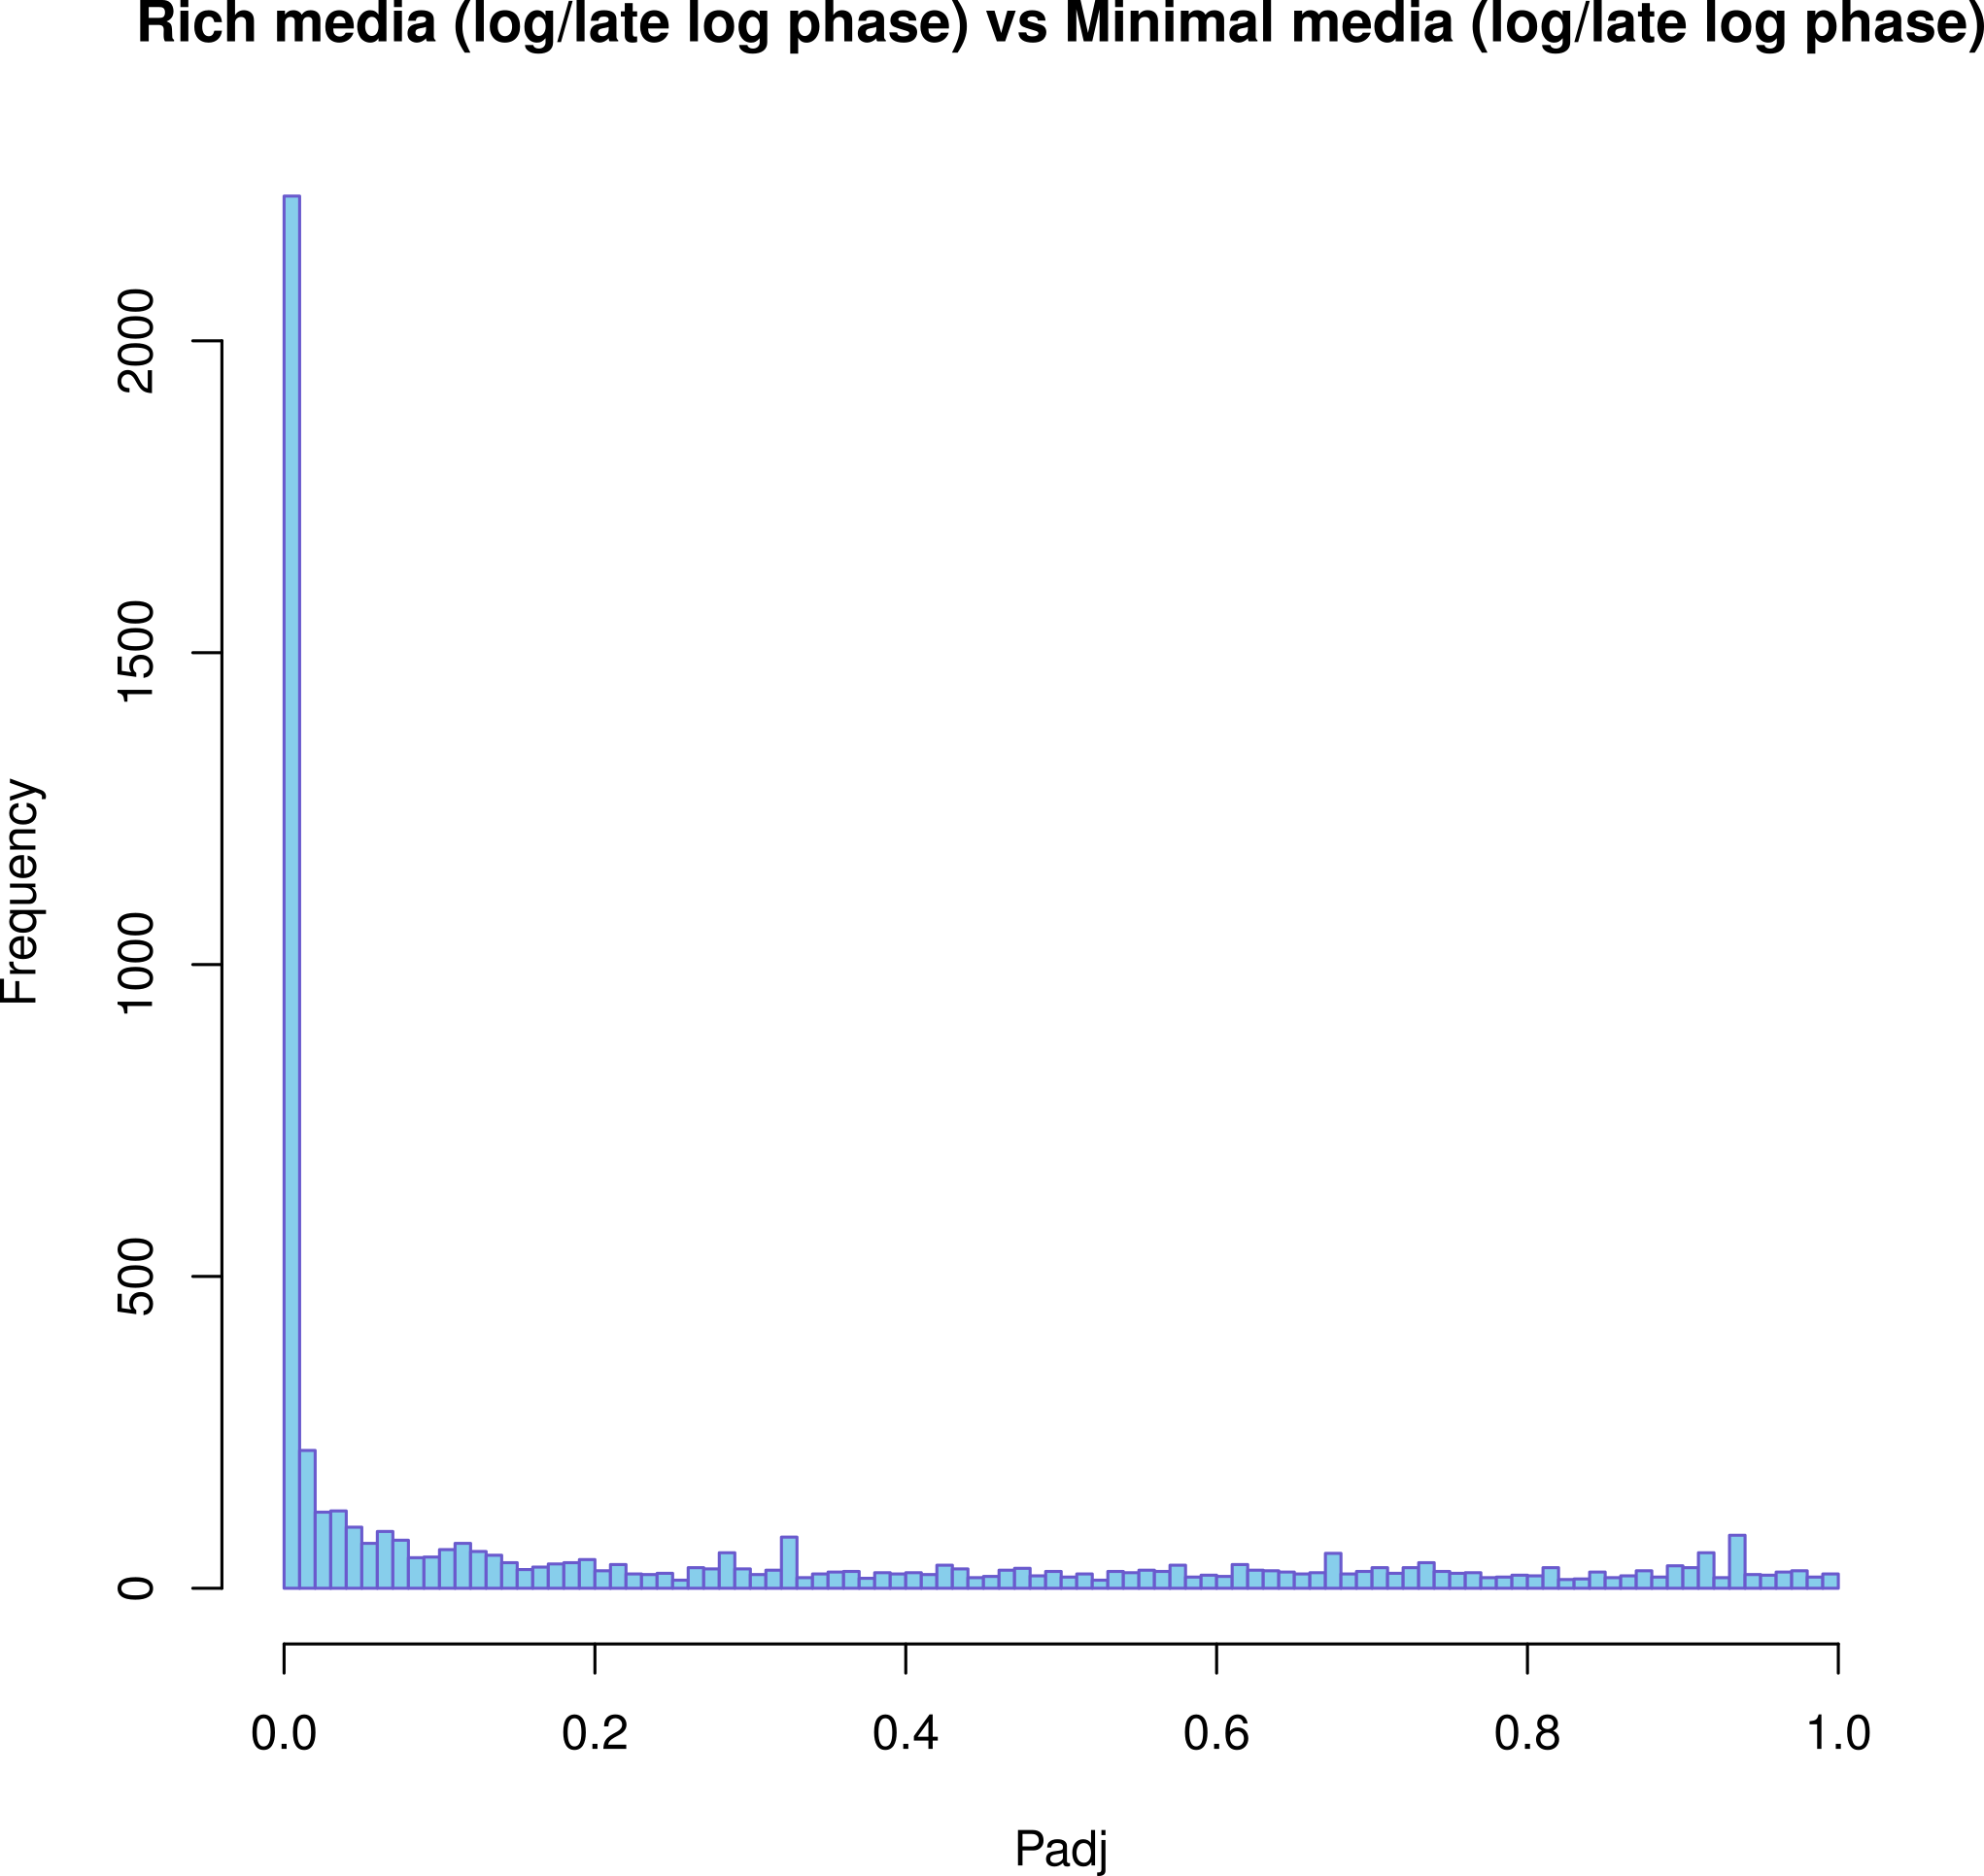
\includegraphics[width=0.9\linewidth]{psa/hist_richloglate_minimal.png}
\end{subfigure}
\begin{minipage}[c]{0.49\textwidth}
\caption[Frequency distributions of P\textsubscript{adj} values for log\textsubscript{2} fold changes for comparisons of growth phases]{Frequency distributions of P\textsubscript{adj} values for log\textsubscript{2} fold changes for pairwise comparisons of growth phases. \textbf{(a)} Rich media, log vs late log. \textbf{(b)} Rich media (log phase) vs Minimal media (log/late log phase) \textbf{(c)} Rich media (log/late log phase) vs Minimal media (log/late log phase). \textbf{(d)} Rich media (log phase) vs starved media (early). \textbf{(e)} Rich media (log/late log phase) vs Minimal media (log/late log phase).}
\label{fig:hist_growth}
  \end{minipage}
\end{figure}

\begin{figure}[H]
\begin{subfigure}{0.5\textwidth}
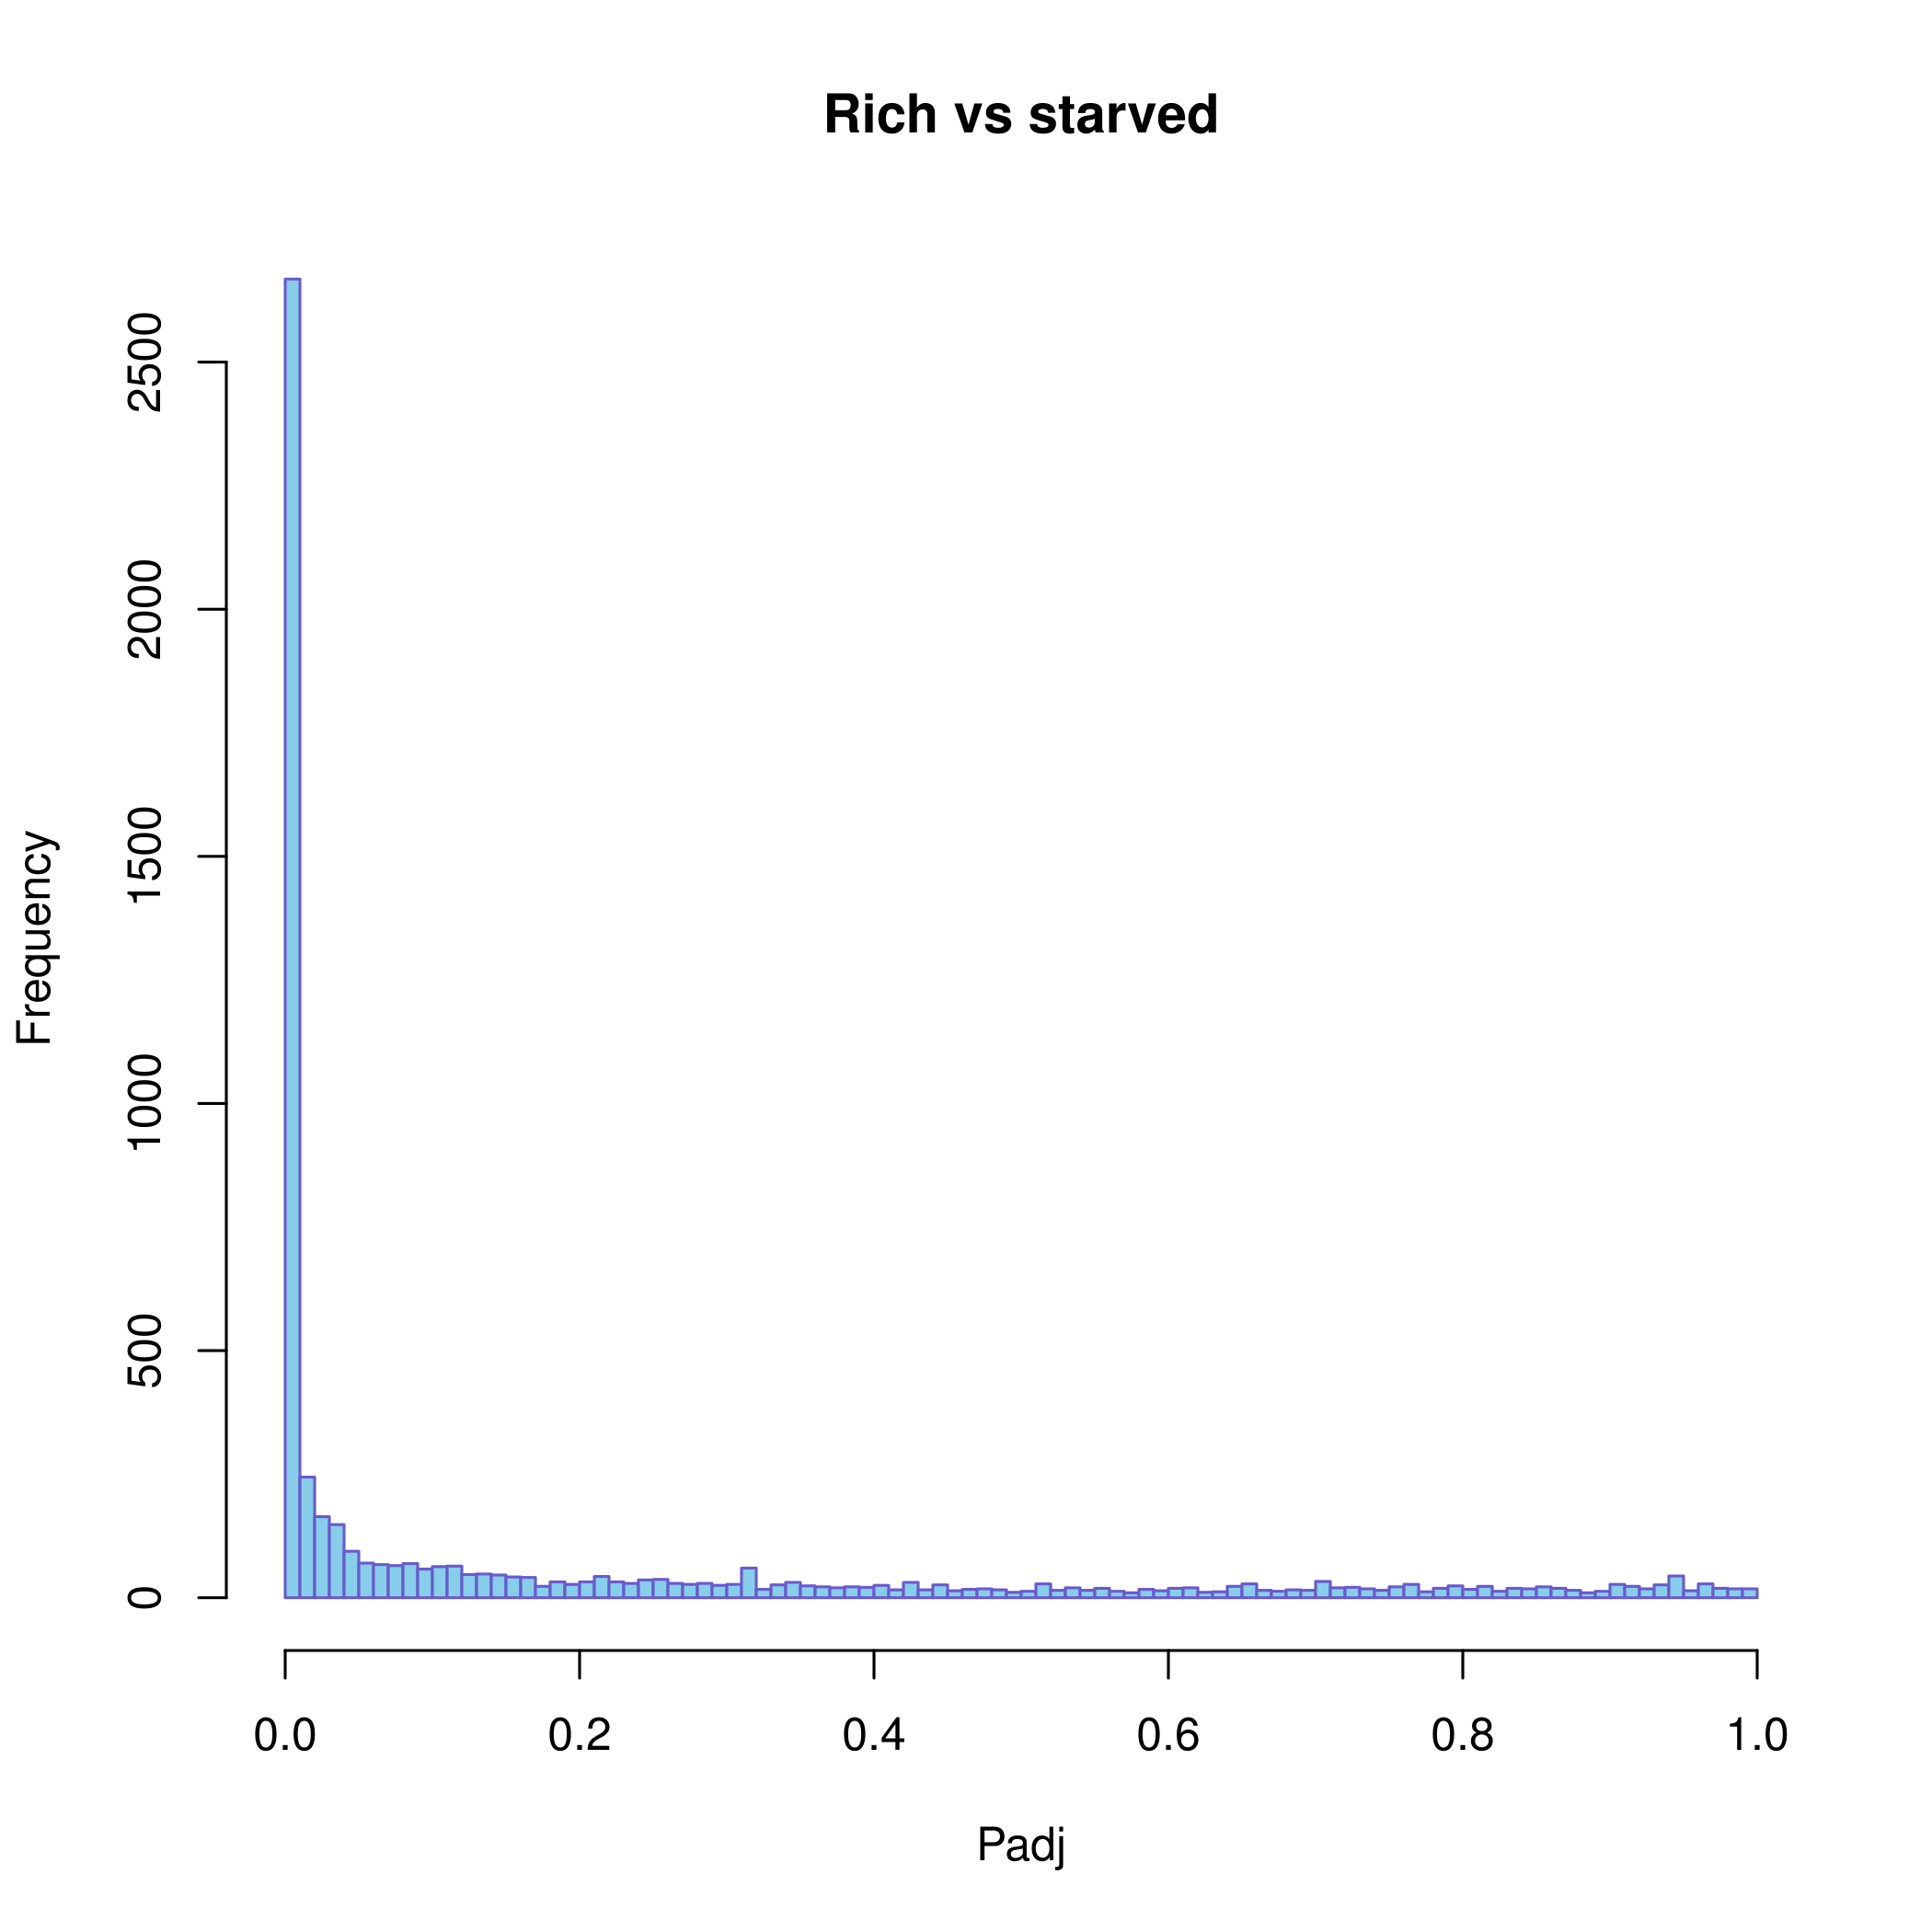
\includegraphics[width=0.9\linewidth]{psa/hist_rich_starved.png} 
\end{subfigure}
\begin{subfigure}{0.5\textwidth}
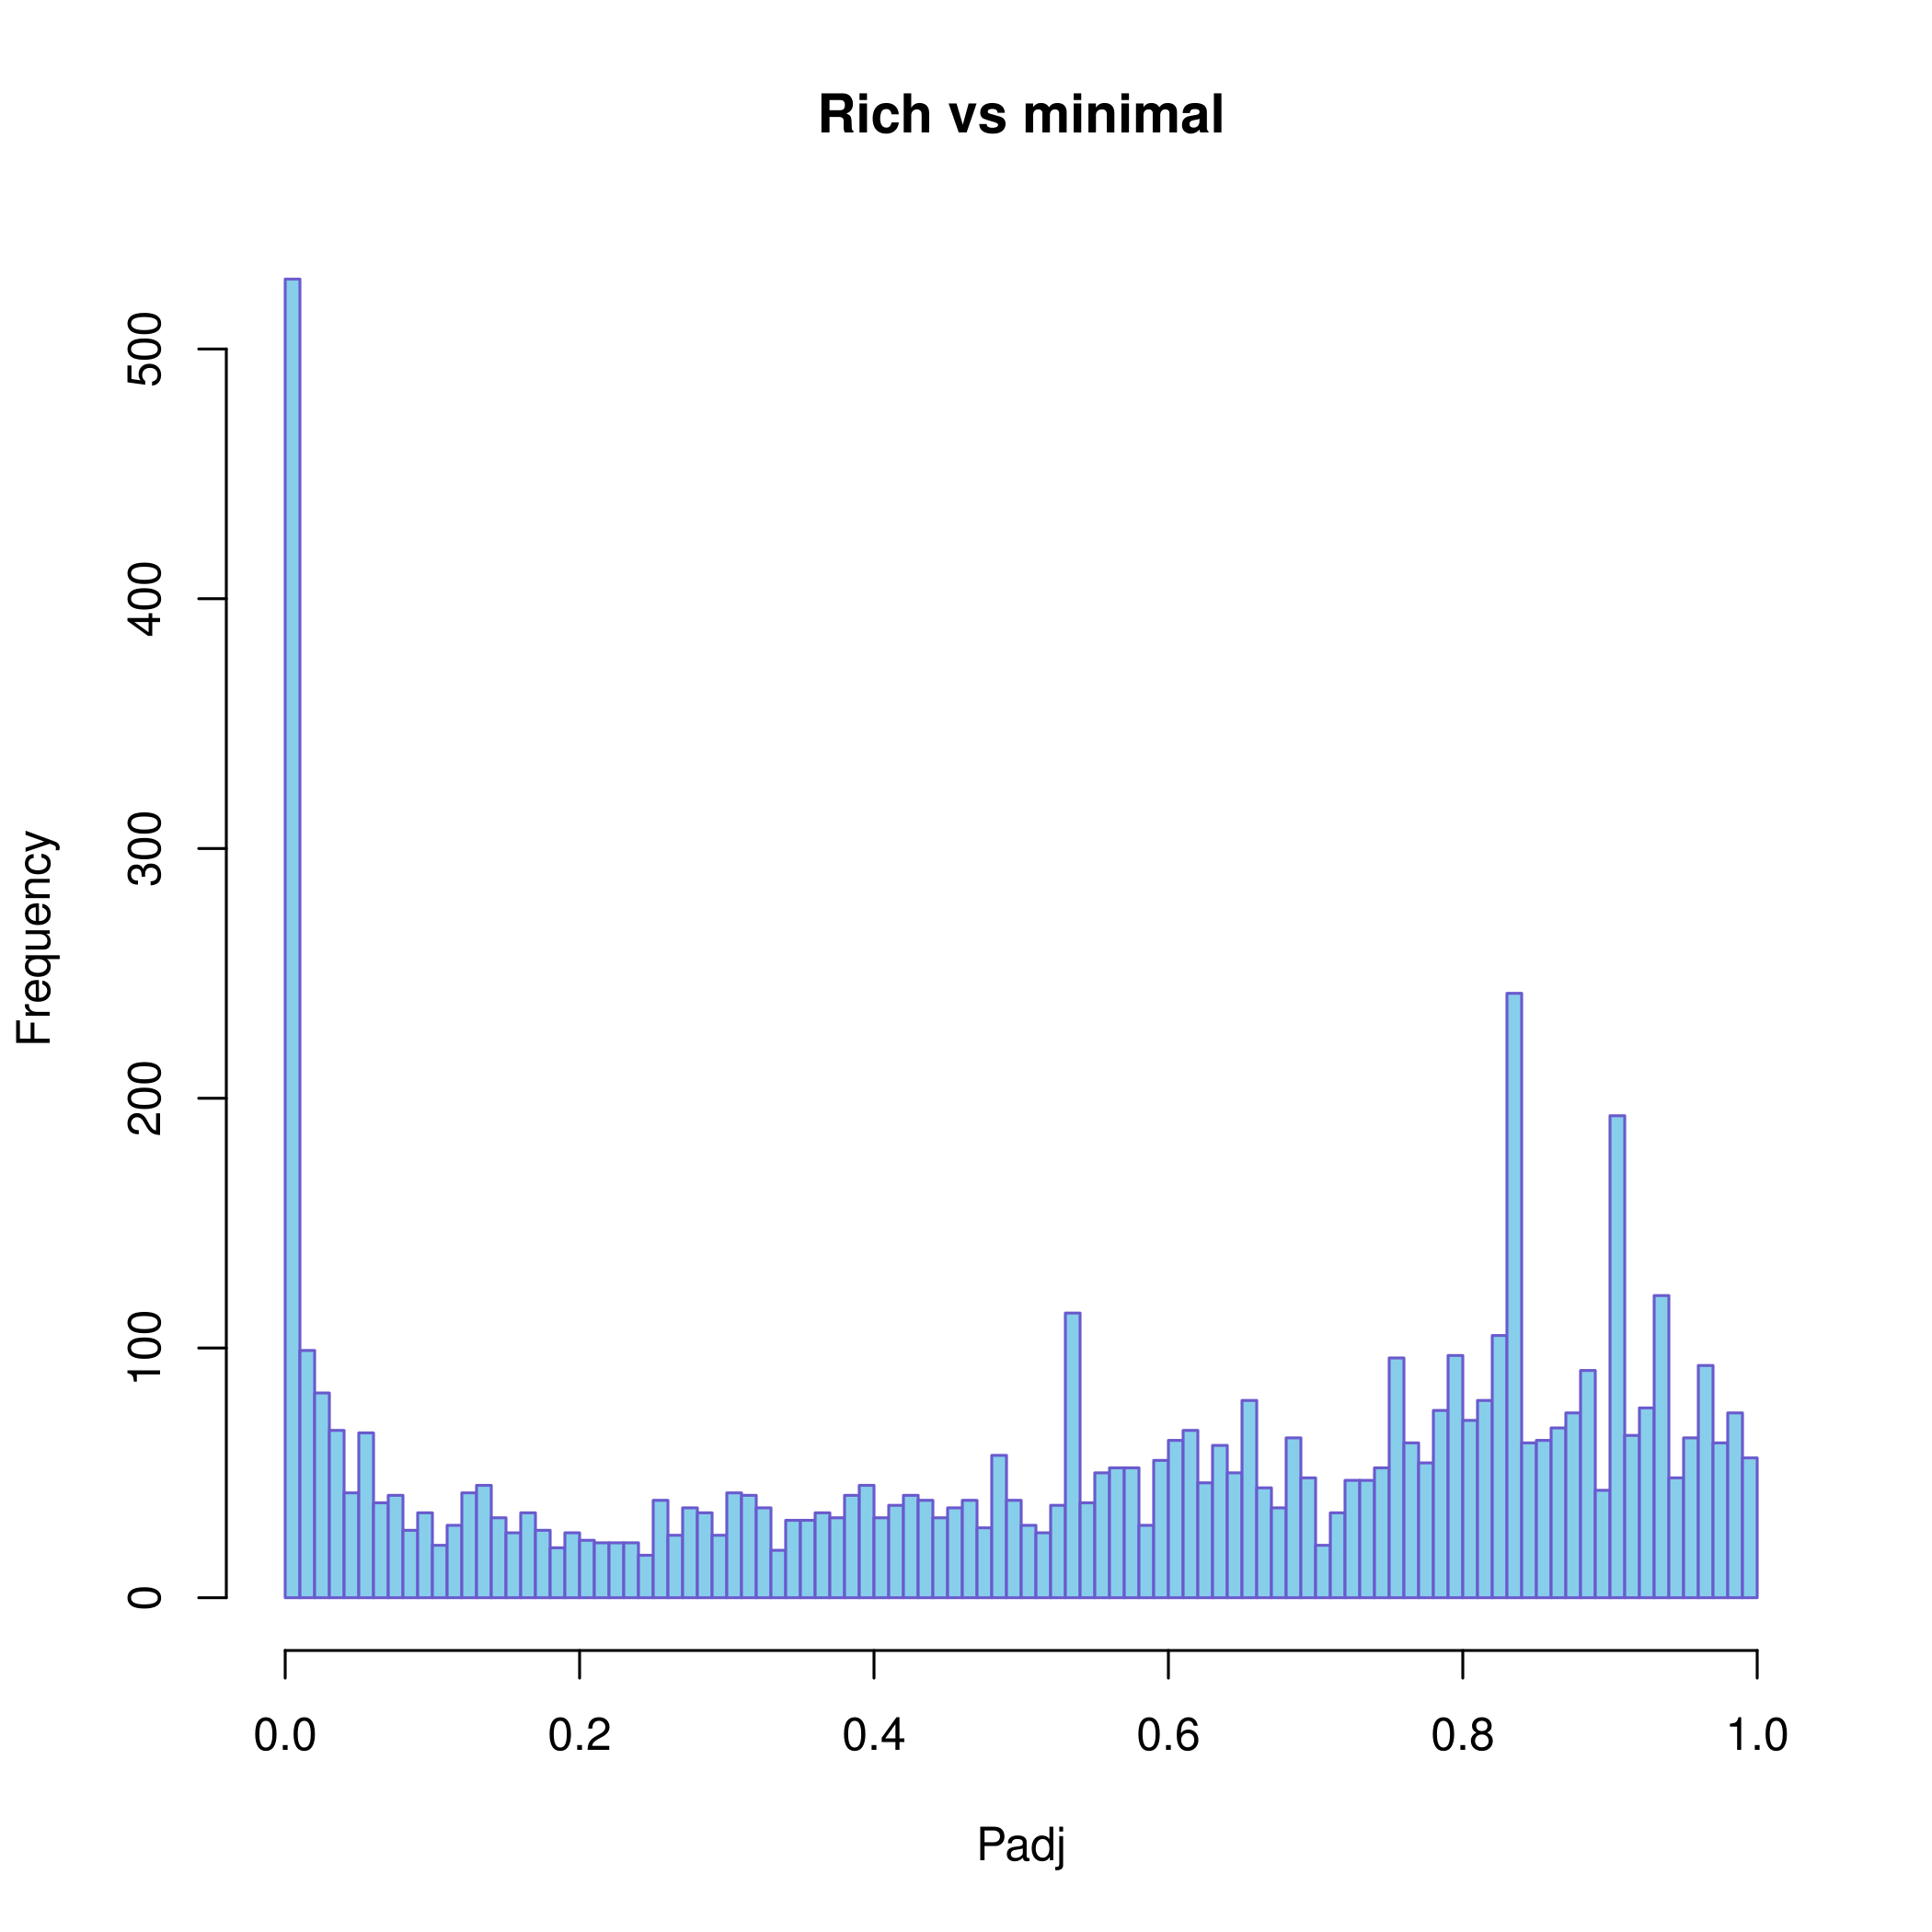
\includegraphics[width=0.9\linewidth]{psa/hist_rich_minimal.png}
\end{subfigure}
\begin{subfigure}{0.5\textwidth}
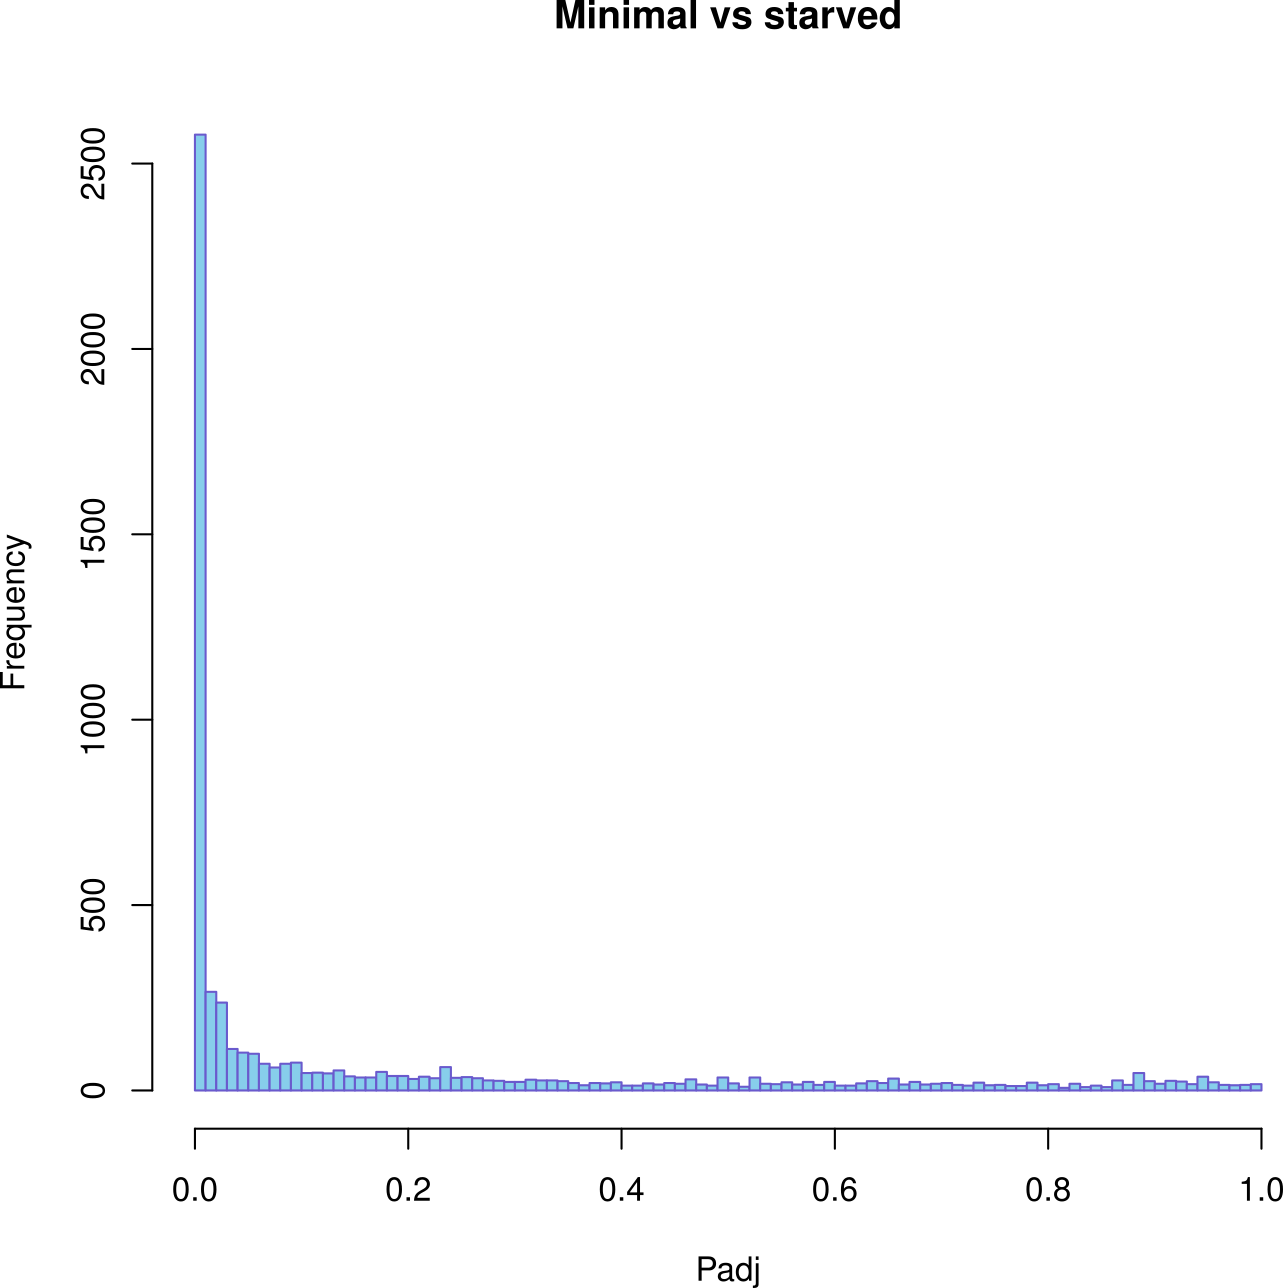
\includegraphics[width=0.9\linewidth]{psa/hist_minimal_starved.png}
\end{subfigure}
\begin{minipage}[c]{0.49\textwidth}
\caption[Frequency distributions of P\textsubscript{adj} values for log\textsubscript{2} fold changes for \textit{in vitro} growth media comparisons]{Histogram showing frequency distributions of P\textsubscript{adj} values for log\textsubscript{2} fold changes for three pairwise comparisons of growth media, \textbf{(a)} Rich vs starved, \textbf{(b)} Rich vs minimal and \textbf{(c)} Minimal vs starved. These comparisons show that most genes are significantly differentially expressed between starved samples and other media types. Comparison between rich vs minimal media samples showed some similarity between samples, as P\textsubscript{adj} values were more evenly distributed.}
\label{fig:hist_media}
  \end{minipage}
\end{figure}

\subsubsection{\textit{In planta} samples}

PCA of all samples showed that the largest contribution to PC1 variance was experiment type (\textit{in planta} and \textit{in vitro}). The top 500 genes with the most variance across the data set (PC1) were inspected to look for major differences in gene expression between the \textit{in planta} and \textit{in vitro} samples. Most of the genes that contribute most to PC1 were effectors and virulence factors that are highly up-regulated in planta. PC2 showed that rich media samples are the most similar to \textit{in planta} samples based on gene expression, and clustered near early infection time-points (1.5hrs, 3hrs, 12hrs and 24hrs post-infection). 

\begin{table}[H]
    \centering
    \begin{tabular}{ccccc}\toprule
    Sample & Sample name & Reads & Total counts & \% Reads mapped to genes \\\midrule
1.5hr & 16 & 38415111 & 179234 & 0.47 \\
1.5hr & 17 & 35889853 & 175850 & 0.49 \\
1.5hr & 20 & 37962490 & 129053 & 0.34 \\
3hr & 25 & 39563552 & 190023 & 0.48 \\
3hr & 26 & 33576040 & 233502 & 0.70 \\
3hr & 27 & 40015335 & 147195 & 0.37 \\
6hr & 28 & 38141276 & 259132 & 0.68 \\
6hr & 29 & 36345675 & 163657 & 0.45 \\
6hr & 30 & 39437965 & 156166 & 0.40 \\
12hr & 34 & 39065761 & 349361 & 0.90 \\
12hr & 37 & 42099962 & 231399 & 0.55 \\
12hr & 38 & 36097446 & 174620 & 0.48 \\
24hr & 3 & 39371740 & 99075 & 0.25 \\
24hr & 41 & 37950153 & 222691 & 0.59 \\
24hr & 42 & 35325178 & 121312 & 0.34 \\
48hr & 10 & 34148479 & 93320 & 0.27 \\
48hr & 43 & 35609939 & 90506 & 0.25 \\
48hr & 44 & 38929993 & 96337 & 0.25 \\
72hr & 12 & 35007764 & 61033 & 0.17 \\
72hr & 6 & 37514121 & 93645 & 0.25 \\
72hr & 8 & 38572996 & 133459 & 0.35 \\
96hr & 55 & 32227055 & 97762 & 0.30 \\
96hr & 56 & 31614369 & 39471 & 0.12 \\
96hr & 57 & 28591692 & 103980 & 0.36 \\
120hr & 49 & 31642015 & 262133 & 0.83 \\
120hr & 50 & 35685140 & 240136 & 0.67 \\
120hr & 51 & 31107467 & 170153 & 0.55 \\
\bottomrule
    \end{tabular}
    \caption[\textit{In planta} read mapping statistics]{Total estimated counts of RNA-seq reads mapping to \textit{Psa} transcripts from \textit{in planta} samples generated by \cite{McAtee2018-sl}.  The overall proportion of reads mapping to \textit{Psa} transcripts for each sample range from 0.12--0.9\%}
    \label{tab:my_label}
\end{table}

\begin{figure}[H]
    \centering
    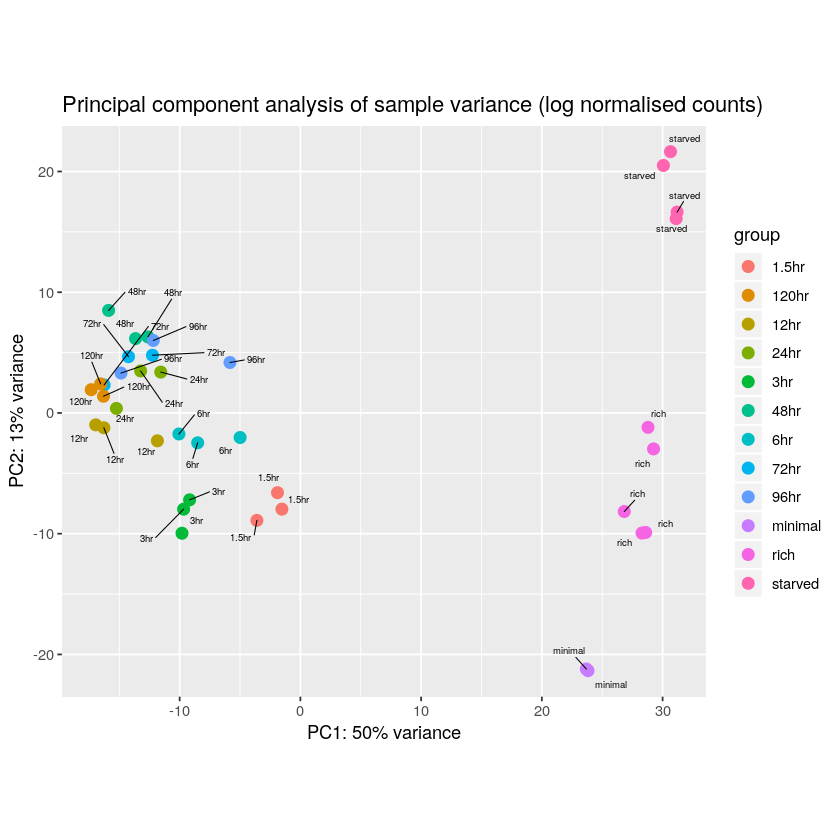
\includegraphics[scale=0.9]{psa/PCA_in_planta.png}
    \caption[PCA plot of \textit{in vitro} and \textit{in planta} samples]{Principal component analysis of gene expression data (log\textsubscript{2} normalised counts) from \textit{in vitro} and \textit{in planta} samples. Sample-sample distances are plotted along the first two principal components (PC1 and PC2). Points represent individual samples, which are coloured by experiment group (\textbf{\textit{In vitro}:} minimal, rich and starved growth mediums. \textbf{\textit{In planta}:} Time-points after \textit{Psa} inoculation on kiwifruit plantlets). The largest variance is between \textit{in vitro} and \textit{in planta} samples, which are separated along PC1, indicating that \textit{in vitro} samples do not mimic \textit{in planta} gene expression. Samples clustered by experiment type along PC1 and PC2, showing similarity between replicates. Sample groups were highly distinct among \textit{in vitro} samples, which were separated along PC2. \textit{In planta} samples were more closely grouped along both PC1 and PC2, with early time-points (1.5hrs-12hrs) showing more variance between each other as well as later time-points. Late time-point \textit{in planta} samples were more closely grouped along PC1 and PC2. \textit{In vitro} rich media samples were similar to early \textit{in planta} time-points along PC2, however, other \textit{in vitro} samples groups were well separated from each other as well as \textit{in planta} samples across both principal components.}
    \label{fig:PCA_in_planta}
\end{figure}

\subsection{Differential gene expression analysis}

\subsubsection{Within \textit{in vitro} comparisons}

Functional annotation of the top 250 DEGs from comparisons between in vitro samples grown in different growth mediums showed the biggest transcriptional changes in genes involved in iron metabolism. Pathway analysis found that most significantly differentially expressed genes were involved in energy metabolism, secondary metabolite biosynthesis and virulence factors (Table \ref{tab:pathway_DEGs}).

\paragraph{Iron homeostasis}

Almost all of the most highly differentially expressed genes in the \textit{in vitro} samples were involved with or dependent on the acquisition and storage of iron. Iron is an essential micro-nutrient for all organisms and is a co-factor in many enzymes, such as those involved in the electron transport chain. For pathogenic bacteria bio-available iron is a major growth limiting factor: most iron in the environment is present as insoluble ferric (Fe\textsuperscript{3+}) iron, and within the host iron may be scarce due to the competing nutritional requirements of the host, or as a defence mechanism \citep{Ratledge2000-qn}. 

Maintaining a suitable balance of iron compounds is important to all cells -- too little iron affects energy production and metabolic capabilities, however free iron can catalyse the production of free radicals \textit{via} Haber-Weiss/Fenton chemistry \citep{Fones2013-vp}. Free ferric iron can react with hydrogen peroxide and superoxide to produce highly reactive hydroxyl ions, which can go on to cause DNA damage by attacking nucleotides \citep{Kehrer2000-ka}. The sequestration of iron is both important to provide nutrients to the bacteria, and as a virulence factor by depriving host cells of iron. Many pseudomonads produce peptide-based siderophore compounds such as pyoverdine, which have higher affinity for ferric than ferrous (Fe$\textsuperscript{2+}$) iron, and are secreted to chelate environmental ferric iron \citep{Cezard2015-ji}. Iron is released from siderophores by a change in affinity by the reduction of ferric iron to ferrous iron. Ferrous iron may then be safely stored as ferric iron by incorporating it into protein-haem complexes such as bacterioferritin \citep{Ratledge2000-qn}.

Bacterioferritin genes were up-regulated in rich media, indicating the stockpiling of abundant free iron. Adaption to iron restriction could be seen in starved and minimal media samples. Siderophore biosynthesis was up-regulated in minimal media (Tables \ref{tab:min_iron}, \ref{tab:min_iron_2}, \ref{tab:min_iron_3}), as were genes involved in iron uptake such as the FagA iron transporter and TonB-dependent outer membrane receptors, which in \textit{Pseudomonas} typically function in siderophore transport and siderophore-induced signal transduction and regulation \citep{lamont-2014}.

{\footnotesize
\begin{longtable}{cl}
    \toprule
    \centering
    \label{tab:pathway_DEGs}
\# DEGs & KEGG pathway number and description \\\midrule
    \endfirsthead
278  & pst01100 - Metabolic pathways \\ 
117  & pst01110 - Biosynthesis of secondary metabolites \\ 
101  & pst01120 - Microbial metabolism in diverse environments \\ 
82  & pst01130 - Biosynthesis of antibiotics \\ 
72  & pst02010 - ABC transporters \\ 
71  & pst02020 - Two-component system \\ 
58  & pst01230 - Biosynthesis of amino acids \\
42  & pst01200 - Carbon metabolism \\ 
32  & pst02024 - Quorum sensing \\ 
27  & pst02030 - Bacterial chemotaxis \\ 
25  & pst00230 - Purine metabolism \\ 
22  & pst02025 - Biofilm formation \\ 
20  & pst00270 - Cysteine and methionine metabolism \\ 
20  & pst00620 - Pyruvate metabolism \\ 
20  & pst00630 - Glyoxylate and dicarboxylate metabolism \\ 
19  & pst00190 - Oxidative phosphorylation \\ 
18  & pst00280 - Valine, leucine and isoleucine degradation \\ 
17  & pst03070 - Bacterial secretion system \\ 
16  & pst00260 - Glycine, serine and threonine metabolism \\ 
16  & pst00650 - Butanoate metabolism \\ 
16  & pst00860 - Porphyrin and chlorophyll metabolism \\ 
16  & pst02040 - Flagellar assembly \\ 
15  & pst00790 - Folate biosynthesis \\ 
15  & pst00920 - Sulfur metabolism \\ 
14  & pst00400 - Phenylalanine, tyrosine and tryptophan biosynthesis \\ 
13  & pst00310 - Lysine degradation \\ 
13  & pst01212 - Fatty acid metabolism \\ 
12  & pst00250 - Alanine, aspartate and glutamate metabolism \\ 
12  & pst00362 - Benzoate degradation \\ 
12  & pst01210 - 2-Oxocarboxylic acid metabolism \\ 
12  & pst03440 - Homologous recombination \\ 
11  & pst00010 - Glycolysis / Gluconeogenesis \\ 
11  & pst00071 - Fatty acid degradation \\ 
11  & pst00220 - Arginine biosynthesis \\ 
10  & pst00240 - Pyrimidine metabolism \\ 
10  & pst00330 - Arginine and proline metabolism \\ 
10  & pst00640 - Propanoate metabolism \\ 
10  & pst00970 - Aminoacyl-tRNA biosynthesis \\ 
    \bottomrule
    \caption[KEGG pathways containing 10 or more significantly DEGs]{KEGG pathways containing 10 or more significantly DEGs from comparisons of \textit{in vitro} trasncriptomes. This is estimated from orthologous genes and pathways from \textit{P. syringae} pv. \textit{tomato} DC3000}
\end{longtable}}

The largest difference between the starved and minimal media samples was the shut-down of siderophore biosynthesis. Although iron is an essential nutritional requirement, siderophores are complex molecules which require large amounts of nitrogen, carbon and ATP to synthesise \citep{Sexton2017-zh}. Starved \textit{Psa} down-regulated genes involved in siderophore biosynthesis and uptake.
\newline

\begin{table}[H]
\footnotesize
    \centering
    \begin{tabular}{p{1.8cm}p{7.5cm}p{0.8cm}p{0.8cm}p{0.8cm}p{1.5cm}}\toprule
Gene & Predicted function & l\textsubscript{2}FC RvS  & l\textsubscript{2}FC RvM & l\textsubscript{2}FC MvS & p\textsubscript{adj} RvM\\\midrule
IYO_010820 & Sigma factor PvdS & 0.26 & 6.81 & -6.55 & 1.81E-07 \\
IYO_010830 & PvdL Pyoverdine chromophore precursor synthetase & 1.28 & 5.56 & -4.29 & 8.67E-12\\
IYO_010840 & Antibiotic synthesis protein MbtH & -0.49 & 4.21 & -4.70 & 1.36E-19\\
IYO_010845 & Metal ABC transporter substrate-binding protein & 1.27 & 4.65 & -3.39 & 4.49E-30\\
IYO_010850 & ABC transporter in pyoverdine gene cluster  & 1.84 & 5.26 & -3.42 & 4.09E-24\\
IYO_010855 & ABC transporter in pyoverdine gene cluster & 1.27 & 4.46 & -3.2 & 7.84E-16 \\
IYO_010880 & Putative iron-regulated membrane protein & 0.93 & 5.41 & -4.48 & 1.69E-14\\
IYO_010885	& SyrP & 0.94 & 6.58 & -5.64 & 4.52E-20\\
IYO_010890 & Pyoverdine sidechain peptide synthetase & 1.28 & 6.35 &-5.07 &2.16E-14\\
IYO_010895 & PvdI Pyoverdine sidechain non-ribosomal peptide synthetase & 1.21 & 5.15 & -3.94 & 1.08E-12\\
IYO_010900 & PvdJ Pyoverdine sidechain non-ribosomal peptide synthetase & 1.83 & 6.28 & -4.45 & 3.84E-27\\
IYO_010905 & PvdD Pyoverdine sidechain non-ribosomal peptide synthetase & 1.84 & 5.22 & -3.38 & 1.87E-15 \\
IYO_011245 & TonB-dependent receptor & -0.29 & 5.89 & -6.18 & 1.21E-29\\ 
IYO_011875 & TonB-dependent receptor & 0.88 & 5.33 &-4.46 &	1.96E-35\\
IYO_012650 & TonB-dependent outer membrane siderophore receptor precursor & 0.47 & 5.21 & -4.73 & 4.69E-29\\
IYO_012660 & PvdE Pyoverdine ABC export system & 1.74 & 6.71 & -4.97 & 2.05E-18\\
IYO_012665 & PvdO Pyoverdine responsive serine/threonine kinase & 1.33 & 6.3 & -4.97 & 1.9E-08\\
IYO_012670 & PvdN Pyoverdine biosynthesis protein & 0.72 & 6.29 & -5.56 & 1.76E-15 \\
IYO_012675 & PvdM Putative pyoverdine biosynthesis dipeptidase & 0.47 & 6.55 & -6.08 & 1.9E-05\\
IYO_012680	& PvdJ/PvdD/PvdP-like protein & -0.51 & 5.56 & -6.07 & 1.86E-19\\
IYO_012685 & Outer membrane pyoverdine eflux protein & 0.95 & 5.17 & -4.22 & 1.6E-48\\
IYO_012690 & Pyoverdine efflux carrier and ATP binding protein & 0.44 & 5.1 & -4.66 & 1.25E-34 \\
\bottomrule
    \end{tabular}
    \caption[Siderophore genes up-regulated in \textit{Psa} in minimal media]{DEGs up-regulated in \textit{Psa} grown in minimal media annotated as being involved in pyoverdine biosynthesis, regulation, and iron transport. L\textsubscript{2}FC is shown for media comparisons: RvS (Rich vs Starved), RvM (Rich vs Minimal) and MvS (Minimal vs Starved). P\textsubscript{adj} is shown for Rich vs Minimal media comparisons.}
    \label{tab:min_iron}
\end{table}

\begin{table}[H]
\footnotesize
    \centering
    \begin{tabular}{p{1.8cm}p{7.5cm}p{0.8cm}p{0.8cm}p{0.8cm}p{1.5cm}}\toprule
Gene & Predicted function & l\textsubscript{2}FC RvS  & l\textsubscript{2}FC RvM & l\textsubscript{2}FC MvS & p\textsubscript{adj} RvM\\\midrule
IYO_013860	& Salicyl-AMP ligase & -0.89 &2.03 &-2.92&1.44E-08\\
IYO_013865	& Yersiniabactin synthesis enzyme YbtT & 0.62 & 3.12 & -2.5&3.15E-13\\															
IYO_013870 &Iron aquisition yersiniabactin synthesis enzyme Irp3 & -0.55 & 2.47 & -3.02 & 1.69E-14\\
IYO_013450 & TonB-dependent ferric achromobactin receptor protein & 0.3 & 3.33 & -3.03 & 6.59E-05\\
IYO_013875 & Iron aquisition yersiniabactin synthesis enzyme Irp1 & 0.89 & 2.66 & -1.77 & 2.37E-07\\
IYO_013885&Iron aquisition yersiniabactin synthesis enzyme Irp2 & 0.05 & 2.67 & -2.62 &8.24E-21 \\
IYO_013900	& Iron aquisition outermembrane yersiniabactin receptor & -0.58 & 5.24 & -5.82 & 3.05E-78\\
\bottomrule
    \end{tabular}
    \caption[Yersiniabactin genes up-regulated in \textit{Psa} in minimal media]{DEGs up-regulated in \textit{Psa} grown in minimal media annotated as being involved in yersiniabactin biosynthesis, regulation, and iron transport. L\textsubscript{2}FC is shown for media comparisons: RvS (Rich vs Starved), RvM (Rich vs Minimal) and MvS (Minimal vs Starved). P\textsubscript{adj} is shown for Rich vs Minimal media comparisons.}
    \label{tab:min_iron_2}
\end{table}

\begin{table}[H]
\footnotesize
    \centering
    \begin{tabular}{p{1.8cm}p{6.5cm}p{0.8cm}p{0.8cm}p{0.8cm}p{1.5cm}}\toprule
Gene & Predicted function & l\textsubscript{2}FC RvS  & l\textsubscript{2}FC RvM & l\textsubscript{2}FC MvS & p\textsubscript{adj} RvM\\\midrule
IYO_013460 &Achromobactin biosynthesis protein AcsD & -0.04 & 2.3 & -2.34 &	9.57E-06\\
IYO_013465	& Achromobactin biosynthesis protein AcsE & -0.24 & 2.62 & -2.85 &	4.88E-17\\
IYO_013475 &Achromobactin biosynthesis protein AcsC & -0.37 & 2.44 & -2.81 & 9.02E-20\\
IYO_013480	& Achromobactin biosynthesis protein AcsB& -0.2 &2.01 &	-2.21 &1.39E-07\\
\bottomrule
    \end{tabular}
    \caption[Achromobactin genes up-regulated in \textit{Psa} in minimal media]{DEGs up-regulated in \textit{Psa} grown in minimal media annotated as being involved in achromobactin biosynthesis, regulation, and iron transport. L\textsubscript{2}FC is shown for media comparisons: RvS (Rich vs Starved), RvM (Rich vs Minimal) and MvS (Minimal vs Starved). P\textsubscript{adj} is shown for Rich vs Minimla media comparisons.}
    \label{tab:min_iron_3}
\end{table}

%Starved \textit{Psa} did however upregulate genes involved in the catabolism of haeme, indicating intra-cellular recycling of iron. https://www.tandfonline.com/doi/abs/10.1179/135100009X392584

\paragraph{Nutritional stress}
%Genes that regulate peptidase (PepSY/M4 proteins) upregulated, peptidases downregulated
\textit{Psa} grown in minimal media and under starvation showed large adaptions to nutrient availability. Genes involved in oxidative phosphorylation were down-regulated and genes involved in the TCA cycle were highly up-regulated in both minimal and starved \textit{Psa} compared to rich media, indicating the induction of carbon metabolism via the Entner-Doudoroff pathway by which pseudomonads utilise carbon sources \citep{Lessie-1984}. 

Glucose metabolism was up-regulated in minimal media compared to other samples (Table \ref{tab:min_glucose}, where glucose was the main carbon source in the media. However \textit{hexR}, which represses glucose metabolism and levansucrase secretion in \textit{P. syringae} \citep{Mehmood_Abdallah_Khandekar_Zhurina_Srivastava_Al-Karablieh_Alfaro-Espinoza_Pletzer_Ullrich_2015}, was also up-regulated, indicating active repression of phosphogluconate metabolism. This may be required for redox balance, as HexR and glucose metabolism are in part controlled by the response to oxidative stress, as well as the intracellular abundance of 2-keto-3-deoxy-6-phosphogluconate \citep{Daddaoua_Krell_Ramos_2009}.

Starved \textit{Psa} up-regulated components of the beta-ketoadipate pathway, which converts cyclic aromatic amino acids to components of the citric acid cycle. One of the most highly expressed genes included phenylalanine hydroxylase (\textit{pheA}), an uncommon step of the pathway present in pseudomonads which converts phenylalanine to tyrosine. 

Many hydroxylases require iron as a cofactor; however, this particular reaction utilises an organic compound, pterin, as a cofactor. Pterin carbinolamine dehydratase, which recycles this pterin cofactor, was also highly up-regulated in starvation conditions. Previous transcriptomic studies of \textit{P. syringae} pv. \textit{syringae} B728a infection in \textit{Arabidopsis} found phenylalanine degradation to be highly up-regulated in epiphytic populations, which may be a pre-emptive response for degrading phenylalanine-based plant defence molecules in the apoplast \citep{Yu-2013}. 
\newline
\begin{table}[H]
\footnotesize
    \centering
    \begin{tabular}{p{1.8cm}p{9cm}p{0.8cm}p{0.8cm}p{0.8cm}}\toprule
Gene & Predicted function & l\textsubscript{2}FC RvS  & l\textsubscript{2}FC RvM & l\textsubscript{2}FC MvS \\\midrule
IYO_006365 & Sugar ABC transporter substrate-binding protein & 1.5 & \textbf{4.37} & -2.88 \\
IYO_006370 & Glucose ABC transport system, inner membrane component 1 & 1.13 & \textbf{4.4} & -3.27\\
IYO_006375 & Glucose ABC transport system, inner membrane component 2 & 0.88 & \textbf{4.13} & \textbf{-3.25}\\
IYO_006380 & Glucose ABC transporter, ATP-binding subunit & 0.71 & 	\textbf{3.63}& \textbf{-2.92}\\
IYO_006390 & Aldose epimerase & -0.65 & \textbf{3.22} & \textbf{-3.87} \\
IYO_006395 & Phosphogluconate repressor HexR & 0.07 & \textbf{1.33} & \textbf{-1.26}\\
IYO_006400 & Glucose-6-phosphate dehydrogenase & -0.27 & \textbf{1.35} & \textbf{-1.62}\\
IYO_006405 & 6-phosphogluconolactonase & 0.4 & \textbf{1.95} & \textbf{-1.55}\\
IYO_006410 & Keto-deoxy-phosphogluconate aldolase & 0.3 & \textbf{2.31} & \textbf{-2.01}\\
\bottomrule
    \end{tabular}
    \caption[DEGs involved in glucose uptake and metabolism up-regulated in \textit{Psa} grown in minimal media]{DEGs up-regulated in \textit{Psa} grown in minimal media annotated as being involved in glucose metabolism, regulation, and transport.  L\textsubscript{2}FC is shown for media comparisons: RvS (Rich vs Starved), RvM (Rich vs Minimal) and MvS (Minimal vs Starved). Fold-changes highlighted in bold are highly significant (p < 0.0001).}
    \label{tab:min_glucose}
\end{table}

PheA was down-regulated in minimal media, as were other components of amino acid degradation. This may be because these pathways are antagonistic to siderophore biosynthesis -- PheA has been found have multiple roles in phenylalanine metabolism, including the degradation of chorismate, which is a key component of pyoverdine siderophores \citep{Molina-2008,Cezard2015-ji}.

Other enzymes involved in secondary metabolic pathways which generate feed-stocks for the TCA cycle, such as enzymes involved in the glyoxylate cycle, were also up-regulated under starvation conditions. This may be due to starved \textit{Psa} utilising peptides from proteins or pyoverdine, or to utilise amino acids in the apoplastic fluid.
\newline
 %extra stuff phenylalanine degradation - component of plant cell walls - also a good carbon source, linked to quorum sensing/signalling "Previous work from our laboratory demonstrated that aromatic amino acids within CF sputum not only serve as carbon and energy sources but also enhance synthesis of the cell signaling molecule PQS (19, 21). " "As expected, genes involved in biosynthesis and response to PQS as well as genes important for catabolism of phenylalanine/tyrosine were highly induced in the presence of aromatic amino acids." https://www.pnas.org/content/110/5/E425 been found to be upregulated in Pseudomonas syringae in epiphytic and apoplast - epiphytic up chemotaxis, produce surfactant, PHENYLALANINE DEGRADATION
 %IYO_009370 phhA Phenylalanine-4-hydroxylase (EC 1.14.16.1) IYO_009375 ATPase AAA Phenylalanine hydroxylase transcriptional activator PhhR

\begin{figure}[H]
    \centering
    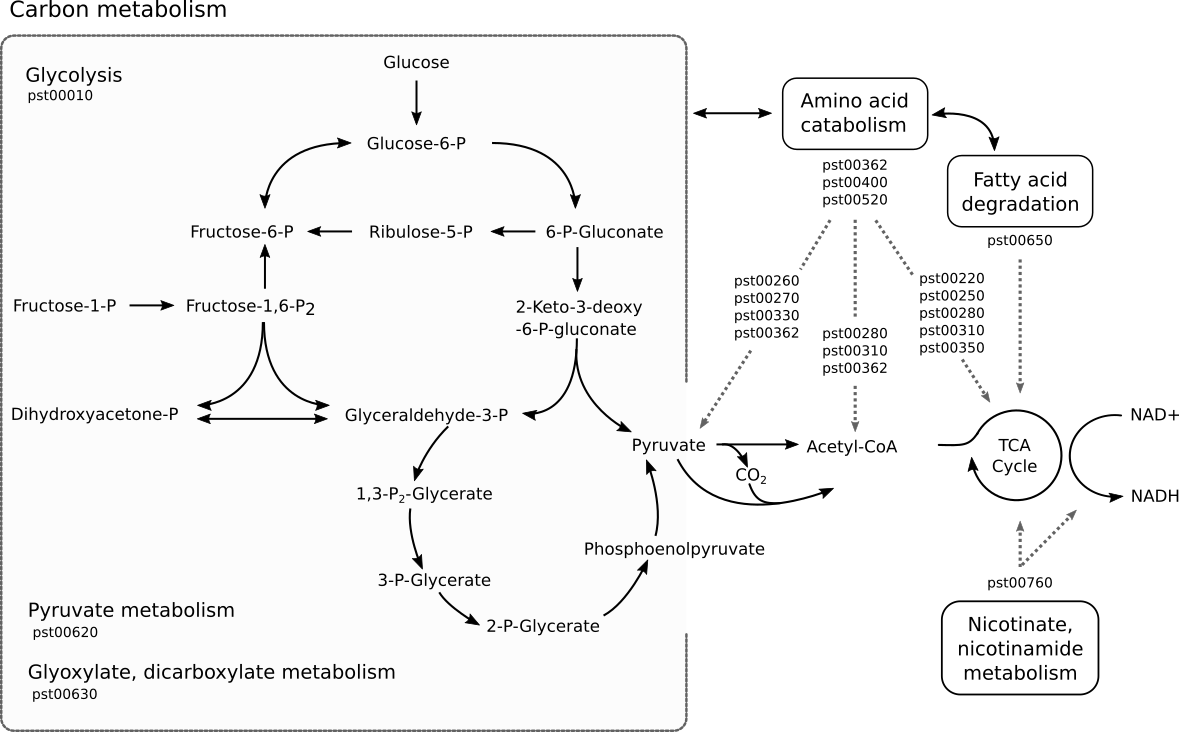
\includegraphics{psa/entner-doudouroff.png}
    \caption[Diagram showing differentially expressed metabolic pathways feeding into energy metabolism in \textit{Psa}]{Diagram showing how differentially expressed KEGG metabolic pathways relate to energy metabolism via the TCA cycle in \textit{Pseudomonas}. Major pathways feeding into the TCA cycle (carbon, amino acid and fatty acid metabolism) are shown contributing carbon feedstocks via pyruvate, acetyl-CoA or as TCA cycle intermediaries. Within carbon metabolism, the Pseudomonas Entner-Doudouroff pathway of hexose sugar metabolism is shown, based on Figure 1 by \cite{Morris1727}. KEGG pathways containing genes that were significantly differentially expressed in the \textit{in vitro} \textit{Psa} RNA-seq are shown as ID numbers (full pathways can be found in Appendix x). }
    \label{fig:entner_doudouroff}
\end{figure}
\paragraph{Redox}

Genes involved in balancing reactive oxygen species were also significantly differentially expressed between sample groups. \textit{P. syringae} and other plant pathogens experience redox stress \textit{in planta} as ROS-generating molecules such as H\textsubscript{2}O\textsubscript{2} are used as a plant defence mechanism \citep{Jones_Lindow_Wildermuth_2007}. Superoxides may also be generated during the extraction of iron from pyoverdine, or generated by reactions with imported free ferric iron. Many genes involved in the electron transport chain also contain iron-sulfur clusters or use iron as cofactors  \citep{Tuanyok_Kim_Nierman_Yu_Dunbar_Moore_Baker_Tom_Ling_Woods_2005}. The down-regulation of genes involved in oxidative phosphorylation, in addition to minimising the use of iron, may also protect the iron-sulphur clusters present in these proteins from oxidative damage \citep{Kawakami_Kuroki_Ishii_Igarashi_Arai_2010}.

Several steps of Entner-Doudouroff metabolic pathways generate NADP\textsuperscript{+}, which can be reduced by ferrodoxins to NADPH, an important co-factor in the oxidative stress response. Many pseudomonads can redirect metabolic pathways towards NADPH production \citep{Kivisaar_2018}, which has been found to promote resistance to oxidative stress in \textit{Pseudomonas putida} \citep{Chavarria_Nikel_Perez-Pantoja_de_Lorenzo_2013}. This could be seen in starved \textit{Psa}, which also up-regulated genes involved in NADP\textsuperscript{+} generation, as well as a ferrodoxin NADP\textsuperscript{+}-reductase. This may be anticipatory of redox stress from plant defence, or to deal with endogenous stress from oxidative degradation of aromatic compounds \citep{Kivisaar_2018}.

The largest fold change between \textit{in vitro} media types were compensatory differences in the gene expression of superoxide dismutase during iron starvation (minimal and starved media), in that those using iron as a co-factor were down-regulated and those using manganese were up-regulated, which has previously been observed in \textit{P. aeruginosa} \citep{Vasil_Ochsner_1999}.

\paragraph{Virulence factors}
\textit{Psa} grown \textit{in vitro} did not express plant-induced \textit{hrp} virulence factors such as the T3SS effectors, which are a major component of the \textit{Psa} transcriptome \textit{in planta} \citep{McAtee2018-sl} (Table \ref{tab:PCA_in_planta_DEGs}). However, in \textit{Psa} grown in minimal media and in starvation conditions, some virulence factors were expressed that may be induced as part of stress responses. 

\textit{Pseudomonas syringae} is able to produce alginate, a polysaccharide composed of mannuronic and guluronic acid. Genes involved in alginate production were slightly up-regulated in minimal and starved compared to rich media, with the most expression in minimal media (Table \ref{tab:alginate}). 
%- summary of DC3000 alginate study These results suggest that signals that precede the HR may stimulate alginate gene expression in P. syringae. Histochemical staining with nitro blue tetrazolium indicated that the superoxide anion () is a signal for algD activation in planta. This study indicates that algD is expressed when P. syringae attempts to colonize both susceptible and resistant plant hosts. \citep{Keith_Keith_Hernández-Guzmán_Uppalapati_Bender_2003}
While alginate biosynthesis was not significantly upregulated in starved \textit{Psa} compared to minimal media, the alginate regulatory components \textit{algU}, \textit{algT} and \textit{algZ} were more highly expressed in starvation conditions, as were several predicted alginate lyases, which are thought to play a role in restructuring alginate polymers \citep{Preston2000-xn}. 

%astra - patterns! RSeP. involved in other
%https://www.ncbi.nlm.nih.gov/pmc/articles/PMC2918974/
These factors were highly expressed independently of the alginate production operon, and have been found to play a role in stress tolerance and virulence and in \textit{P. syringae} \citep{Schurr_Yu_Martinez-Salazar_Boucher_Deretic_1996,Schenk_Weingart_Ullrich_2008,Keith_Bender_1999,Baynham_Brown_Hall_Wozniak_1999}. The carbon storage regulator \textit{csrA} was highly up-regulated in starved \textit{Psa}, which in \textit{P. syringae} pv. \textit{tomato} DC3000 can control virulence expression, including the repression of alginate production \citep{Ferreiro_Nogales_Farias_Olmedilla_Sanjuan_Gallegos_2018}.
\begin{table}[H]
\footnotesize
    \centering
    \begin{tabular}{p{1.8cm}p{8cm}p{0.8cm}p{0.8cm}p{0.8cm}}\toprule
Gene & Predicted function & l\textsubscript{2}FC RvS  & l\textsubscript{2}FC RvM & l\textsubscript{2}FC MvS \\\midrule
IYO_006020 & Alginate o-acetyltransferase AlgF & -0.01 & \textbf{1.05} & \textbf{-1.05}\\
IYO_006035 & AlgL Alginate lyase precursor & \textbf{1.15} & \textbf{1.48} & -0.33\\
IYO_006040 & Alginate O-acetyltransferase AlgX & -0.1 & \textbf{1.2} &\textbf{-1.3}\\
IYO_006045 & Poly(beta-D-mannuronate) C5 epimerase & 0.7 & \textbf{1.65} &	\textbf{-0.94}\\
IYO_006050 & alginate regulatory protein AlgE & 0.67 & \textbf{1.98} & \textbf{-1.31}\\	
IYO_006055 & Alginate biosynthesis protein AlgK precursor & \textbf{0.99} & \textbf{1.86} & -0.88 \\
IYO_006060 & Alginate biosynthesis protein Alg44 & 0.59 & \textbf{1.73} & \textbf{-1.14} \\	
IYO_006065 & Glycosyl transferase	Alginate biosynthesis protein Alg8 &1.01 & \textbf{2.96} & \textbf{-1.95} \\
IYO_006070	& GDP-mannose 6-dehydrogenase & \textbf{1.41} & \textbf{3.2} & \textbf{-1.79}\\	
IYO_021520	& RNA polymerase sigma-H factor AlgU & \textbf{1.68} & 0.32 & \textbf{1.35}\\
IYO_021530	& RNA polymerase sigma-H factor AlgT & \textbf{1.25} & 0.03 & 1.22
\\
IYO_000530	& Alginate biosynthesis protein AlgZ/FimS & \textbf{2.84} & -0.7 & \textbf{3.53} \\
IYO_001890	& Alginate biosynthesis transcriptional regulator AlgB	& \textbf{1.20} & -0.30 & \textbf{1.50}\\
\bottomrule
    \end{tabular}
    \caption[DEGs involved in alginate biosynthesis]{DEGs up-regulated in \textit{Psa} annotated as being involved in alginate biosynthesis. Log\textsubscript{2} fold-change is shown for each gene in for each pairwise media comparison. L\textsubscript{2}FC is shown for media comparisons: RvS (Rich vs Starved), RvM (Rich vs Minimal) and MvS (Minimal vs Starved).  Fold-changes highlighted in bold are significant (p < 0.0001).}
    \label{tab:alginate}
\end{table}

Starved \textit{Psa} up-regulated virulence factors involved in survival in ephiphytic environments, such as motility, chemotaxis and adhesion \citep{Lindow_Andersen_Beattie_1993}. 
Chemotaxis and flagella biosynthesis were up-regulated in starvation conditions, as were components of the type III secretion system, however the respective effectors were down-regulated, suggesting this may be involved with the transport of the flagellar components \citep{Diepold_Armitage_2015}.

As well as the characteristic type III secretion system, \textit{Psa} genomes contain components of type I, II, IV and VI secretion systems \citep{Marcelletti_Ferrante_Petriccione_Firrao_Scortichini_2011}. Genes annotated as components of type VI, II and IV secretion systems were all down-regulated in starved \textit{Psa}. The function of these systems in \textit{Psa} are not well characterised, but are often found to have roles in effector and toxin secretion in pathogens \citep{Records_Gross_2010,Marcelletti_Ferrante_Petriccione_Firrao_Scortichini_2011}. One exception was a gene annotated as type V Aida, which is thought to be involved in adherence \citep{Henderson_2004}. Other genes which contribute to virulence and survival such as pili and fibriae were also up-regulated under starvation conditions. 

Antibiotic resistance mechanisms were also up-regulated in starved \textit{Psa}. An operon containing beta-lactamase (IYO\textunderscore000615) and multidrug transporter genes was found to be highly up-regulated. Genes with beta-lactamase activities were down-regulated in minimal media, which may be to prevent degradation of secondary metabolites produced by \textit{Psa}.

\textit{Psa} genomes contains a multitude of transposons, group II introns and other mobile genetic elements, which are thought to contribute to their high genetic diversity. Many of these elements are highly multi-copy, making it difficult to quantify changes in gene expression for individual genes. Of the mobile genetic elements that were single-copy, several integrases and tyrosine recombinases were up-regulated in starved \textit{Psa}
% IYO_029910 integrase XerC superfamily Tyrosine recombinase XerC IYO_017050 integrase Cointegrate resolution protein T IYO_023220 integrase Mobile element protein
\subsubsection{Comparison between \textit{Psa} grown \textit{in planta} and \textit{in vitro}}

Comparison of the \textit{in vitro} and \textit{in planta} experiments found that \textit{in planta} experiments showed increased expression of the HrpL alternative \textsigma -factor, which binds to the promoter region of \textit{hrp}-genes \citep{Fouts2002-ev}, as were the type III secretion system effectors that are part of the HrpL regulon (Table \ref{tab:PCA_in_planta_DEGs}). This reflects observations by previous studies, which show that \textit{hrp}-regulated genes are not expressed in minimal media without additional stressors such as changes in pH and osmolyte content \citep{McAtee2018-sl,Rahme_Mindrinos_Panopoulos_1992}. 
%Induced in vitro expression of hrp-genes has been found to be substantially lower than \textit{in planta}, highlighting the importance of plant environmental signals on \textit{hrp}-gene regulation \citep{Rahme_Mindrinos_Panopoulos_1992}. 

Principal component analysis (Figure \ref{fig:PCA_in_planta}) showed that these genes contributed the most to PC1, which clustered samples by experiment type, indicating that the induction of effectors and virulence factors \textit{in planta} was the biggest difference between the \textit{in vitro} and \textit{in planta} transcriptomes. Effector genes were among the most abundant transcripts in \textit{in planta} samples, and had higher read counts in \textit{in planta} samples than \textit{in vitro} samples prior to normalisation, despite the \textasciitilde 100-fold in sample read depth between the two experiment types.

The \textit{in vitro} experiments in this study primarily capture transcriptional changes in response to nutrient availability.  \textit{In vitro} experiments showed similarities to several previous comparisons of \textit{in vitro} and \textit{in planta} \textit{Psa} transcriptomes, and are not necessarily analogous to a particular stage of infection. 

The PCA plot for \textit{in vitro} and \textit{in planta} samples (Figure \ref{fig:PCA_in_planta}) showed that early time-points (1.5--12hrs) clustered with samples grown in rich media along PC2. Overall, \textit{hrp}-genes were among the most significantly differentially expressed genes in comparisons between \textit{Psa} grown \textit{in planta} and \textit{in vitro} in rich media (Table \ref{tab:vitro_v_planta}). \cite{McAtee2018-sl} found that fewer of these genes were expressed in early time-points, which may explain the closer association of rich media samples with these time-points. 

\begin{table}[H]
    \centering
    \begin{tabular}{cccl}\toprule
Gene & PC1 contribution & L\textsubscript{2}FC & Annotation \\\midrule
IYO_015535 & 1.00 & 11.77 & hypothetical protein\\
IYO_005980 & 0.85 & 8.44 & *\\
IYO_001355	& 0.85	& 8.44	& * \\
IYO_027300	& 0.85	& 8.44	& * \\
IYO_000990	& 0.85	& 8.44	& * \\
IYO_027930	& 0.85	& 8.44	& * \\
IYO_006790	& 0.85	& 8.38	& Type III secretion HrpA pilin\\
IYO_006750	& 0.80	& 8.38	& type III effector HrpW1 with pectin lyase domain\\
IYO_022020	& 0.79	& 8.24	& hemolysin\\
IYO_015990	& 0.77	& 8.60	& membrane protein\\
IYO_022025	& 0.77	& 8.72	& glycerol acyltransferase\\
IYO_002645	& 0.71	& 10.02	& * \\
IYO_003480	& 0.71	& 10.02	& * \\
IYO_011415	& 0.71	& 10.02	& * \\
IYO_028495	& 0.71	& 10.02	& * \\
IYO_023550	& 0.71	& 10.02	& * \\
IYO_000975	& 0.67	& 9.24	& hypothetical protein \\
IYO_028770	& 0.66	& 6.82	& LysR family transcriptional regulator \\
IYO_008385	& 0.64	& 7.14	& hopAM1-2 \\
IYO_023205	& 0.64	& 7.14	& hopAM1-1 \\
IYO_017375	& 0.61	& 7.98	& Phosphonate ABC transporter \\
IYO_014970	& 0.57	& 6.60	& hypothetical protein \\
IYO_005100	& 0.56	& 6.58	& hypothetical protein \\
IYO_027905	& 0.54	& 6.15	& Organosulfonate utilization protein SsuF \\
IYO_006735	& 0.54	& 6.11	& hopN1 \\
IYO_006880	& 0.54	& 6.76	& type III secretion protein \\
IYO_026605	& 0.53&	6.13	& monooxygenase \\
IYO_006820	& 0.53	& 5.94	& type III secretion protein HrpF \\
IYO_011995	& 0.52 & 6.03	& phosphate ABC transporter substrate-binding protein \\
IYO_011310	& 0.51	& 6.28	& NAD(P)H-dependent FMN reductase \\
    \end{tabular}
    \caption[Genes contributing to variance of principal component 1 in \textit{in vitro} and \textit{in planta} transcriptome comparison]{Top 30 genes contributing to PC1 variance in Figure \ref{fig:PCA_in_planta}. L\textsubscript{2}FC \textit{in planta} compared to \textit{in vitro} and functional annotation are also shown (* denotes multi-copy transposons). The majority of these genes are hrp-controlled components of the type III secretion system and hop (Hrp-dependent outer protein) effectors.}
    \label{tab:PCA_in_planta_DEGs}
\end{table}
\newpage
Despite similarities between rich media and \textit{in planta} samples, minimal media samples had the fewest significantly expressed genes of the \textit{in vitro} samples (Table \ref{tab:sig_DEGs_planta}. Comparisons of rich and minimal media with \textit{in planta} samples indicate that \textit{Psa} nutrition \textit{in planta} is well supported, however, similarities with minimal media samples indicate that stress responses are overall more highly expressed \textit{in planta}. Siderophore synthesis was significantly up-regulated in minimal media, despite the weak expression of these genes \textit{in planta} \citep{McAtee2018-sl}. Other differentially expressed genes relative to rich media included proteins involved in ion and sulfonate transport, which were more highly expressed \textit{in planta}.

 \hfill
\begin{table}[H]
    \centering
    \begin{tabular}{cc}\toprule
Media type & \# DEGs  compared to \textit{in planta} samples\\\midrule
Starved  & 2194 \\
Minimal & 1237 \\
Rich  & 2045 \\\bottomrule
    \end{tabular}
    \caption[Numbers of significantly expressed genes for \textit{in vitro} sample comparisons]{Numbers of highly differentially expressed genes for pairwise comparisons of \textit{in vitro} samples in different growth medias with \textit{in planta} samples (P\textsubscript{adj} < 0.0001)	}
    \label{tab:sig_DEGs_planta}
\end{table}

M9 media has traditionally been used to simulate the nutritional profile of apoplastic fluid in studies of metabolic adaptions of \textit{P. syringae} pathovars during early infection \citep{Rahme_Mindrinos_Panopoulos_1992, OLeary_Neale_Geilfus_Jackson_Arnold_Preston_2016}. However, this does not entirely capture nutritional changes that may occur within the apoplast due to bacterial consumption of resources, as well as responses from the plant intended to restrict bacterial growth. For example, many genes involved in response to nutritional stress have been found to be down-regulated by \textit{P. syringae} pv. \textit{phaseolicola} grown in leaf and apoplastic fluid extracts compared to an M9 minimal media control \cite{Hernandez-Morales_De}. \textit{P. syringae} pathovars are adapted to utilise sugars and carbohydrates in the apoplast \citep{Rico2008-of}, and preferred substrates such as amino acids and dicarboxylates are also found in high concentrations in apoplastic fluids  \citep{OLeary_Neale_Geilfus_Jackson_Arnold_Preston_2016}. 

\textit{Psa} grown in minimal media and under starvation conditions showed large-scale transcriptional changes to adapt to nutritional stress and iron restriction. With the exception of effectors, transcriptional differences found by \cite{Yu-2013}'s comparison of \textit{P. syringae} B728a in epiphytic vs apoplastic sites were similar to changes in \textit{Psa} gene expression between starved and minimal media \textit{in vitro} samples. \textit{Psa} may also experience starvation within the plant as well as on the surface, as local resources are exhausted. Metabolic adaptions seen in starved \textit{Psa}, where the Entner-Doudoroff pathway and TCA cycle were up-regulated, was also seen in \textit{P. syringae} pv. \textit{phaseolicola} in apoplastic fluid after all preferred carbon sources were consumed in apoplastic fluid \citep{OLeary_Neale_Geilfus_Jackson_Arnold_Preston_2016}. 

{\footnotesize
\begin{longtable}{p{2cm}p{2cm}p{9cm}p{1cm}}
    \toprule
    \centering
Comparison with \textit{in planta} & Gene & Predicted function & l\textsubscript{2}FC\\\midrule
\endfirsthead
Starved & IYO_015535 & Hypothetical protein & 10.86\\
&IYO_005475 & Membrane protein & -5.19 \\
&IYO_000485 & Transposase & -2.84\\
&IYO_001195 & Transposase  & -2.84\\
&IYO_001615 & Transposase & -2.84\\
&IYO_001730 & Transposase & -2.84\\
&IYO_005000 & Transposase & -2.84\\
&IYO_009075 & Transposase & -2.84\\
&IYO_012240 & Transposase & -2.84\\
&IYO_013520 & Transposase & -2.84\\
Minimal& IYO_015535 & Hypothetical protein & 12.31\\
&IYO_006735 & HopN1 & 6.35\\
&IYO_021635 & Hypothetical protein & 5.72\\
&IYO_004250 & Hypothetical protein & 5.05\\
&IYO_014970 & Hypothetical protein & 6\\
&IYO_006730 &  Type III chaperone protein ShcN & 5.37\\
&IYO_005100 & Hypothetical protein & 6.86\\
&IYO_029645 & LuxR family transcriptional regulator & 3.98\\
&IYO_012700 & Acyl-homoserine lactone acylase PvdQ & -5.69\\
Rich &IYO_015535 & Hypothetical protein & 12.6\\
&IYO_006735 & HopN1 & 6.63\\
&IYO_021635 & Hypothetical protein & 5.76\\
&IYO_014970 & Hypothetical protein & 6.77\\
&IYO_006730  & Type III chaperone protein ShcN & 6.2\\
&IYO_004250 & Hypothetical protein & 4.8\\
&IYO_005100 & Hypothetical protein & 7.63\\
&IYO_006790  & Type III secretion HrpA pilin & 8.71\\
&IYO_010735 & Hypothetical protein & 4.69\\
&IYO_029700 & Hypothetical protein & 5.57\\

\bottomrule
    \caption[Top 10 differentially expressed genes between \textit{in planta} and \textit{in vitro} transcriptomes]{Top 10 DEGs from comparisons of all \textit{in planta} transcriptomes to \textit{in vitro} samples  different growth media (starved, minimal and rich). DEGs are chosen by the smallest P\textsubscript{adj} value, which are all below 1x10\textsuperscript{-50}. Log\textsubscript{2} fold change \textit{in planta} relative to \textit{in vitro} is shown. }
    \label{tab:vitro_v_planta}
\end{longtable}}
Genes involved in alginate and extracellular polysaccharide biosynthesis and secretion expressed \textit{in vitro} in minimal media and under starvation were also up-regulated expressed at late time-points \textit{in planta} \citep{McAtee2018-sl}. However, the role of these compounds in virulence and ephiphytic survival remains unclear. 

\section{Conclusions and future directions}

The ability to adapt to changeable and hostile environments is a major contributor to the success of pathogenic bacteria. \textit{Psa} encounters several extreme environments and challenges during its life course, and must adapt its metabolism and homeostatic mechanisms appropriately. We present a high-depth RNA-seq dataset of the kiwifruit pathogen \textit{Psa} grown \textit{in vitro} in multiple growth media. Comparisons of these transcriptomes shows large-scale adaptions to cope with drastic changes in nutrient availability. These data also found that starvation conditions triggered several anticipatory responses to plant defence mechanisms, highlighting the regulatory connections between metabolism and virulence. 

%While mobile genetic elements that contribute to the genomic diversity of \textit{Psa} are difficult to study individually, increased expression of elements that are likely to contribute to horizontal gene transfer and genomic rearrangements in starved \textit{Psa}. 
While the \textit{in vitro} data generated for this chapter did not induce the expression of many gene cohorts found to be highly expressed \textit{in planta} \citep{McAtee2018-sl}, these data show that \textit{Psa} grown \textit{in vitro} in nutrient-limiting conditions has similar transcriptional responses as other \textit{P. syringae} pathovars in apoplastic and epiphytic environments. Methods for transposon insertion sequencing experiments in \textit{Psa} are currently being developed \citep{Mesarich2017-ad}, which will provide a measure of gene essentiality for specific growth conditions. Current methods for dual RNA-seq studies of bacterial pathogens \textit{in planta} are more challenging to perform than in animal cell lines, and have low bacterial transcript yields from plant tissue\citep{Nobori2018-uu}. Identifying analogous \textit{in vitro} growth conditions will allow us to identify and isolate environmental signals and stressors that trigger the expression of virulence genes, or other changes in gene expression important for survival.

\bibliographystyle{otago}
\bibliography{psa_RNAseq}